\documentclass[a4paper,12pt,english]{memoir}
\usepackage{babel}
\usepackage{listings}
\usepackage{graphicx}
\usepackage{amsmath}

\newcommand{\tx}{\textit{tx}}
%\newcommand{{\concat}{$\mathbin\Vert$}
\DeclareMathOperator{\concat}{\mathbin\Vert}

\title{Corda ZKNotary}


\begin{document}

\maketitle

% use optional argument because the \LaTeX command breaks the PDF keywords
\chapterstyle{bianchi}

\begin{abstract}

\end{abstract}

\chapter*{Introduction}

\begin{itemize}
\item Brief introduction to Corda
\item Problem statement
\end{itemize}


\chapter*{Design Choices}

\subsection{Transaction representation:Merkle Tree vs Concatenation}

\subsection{Selection of Nonce for ZKStateRef}

\textbf{Problem:} ZKStateRef can be computed as $\text{ZKStateRef} = Hash(\text{Transaction State})$.
However, this computation is not resistant to pre-image attacks and collisions.

A solution to this problem is adding a nonce in computation such that $\text{ZKStateRef} = Hash(\text{nonce} \concat \text{Transaction State})$, which can prevent such attacks.
However, generating a nonce in Corda requires to perform a hash operation which is a costly operation in ZK circuits.
As an alternative, \textit{can we use the same nonce that is generated for the hashing of component elements?}

Before answering this question, we provide some information about the data that is used in the computation of ZKStateRef.
We compute ZKStateRef for input, output, and reference components.
Each element in these component groups are a \texttt{ZKStateAndRef} object which consists of a \texttt{Transaction State} and \texttt{ZKStateRef}.
Figure~\ref{fig:tree_ts} shows the relation between each object.

\begin{figure}[ht]
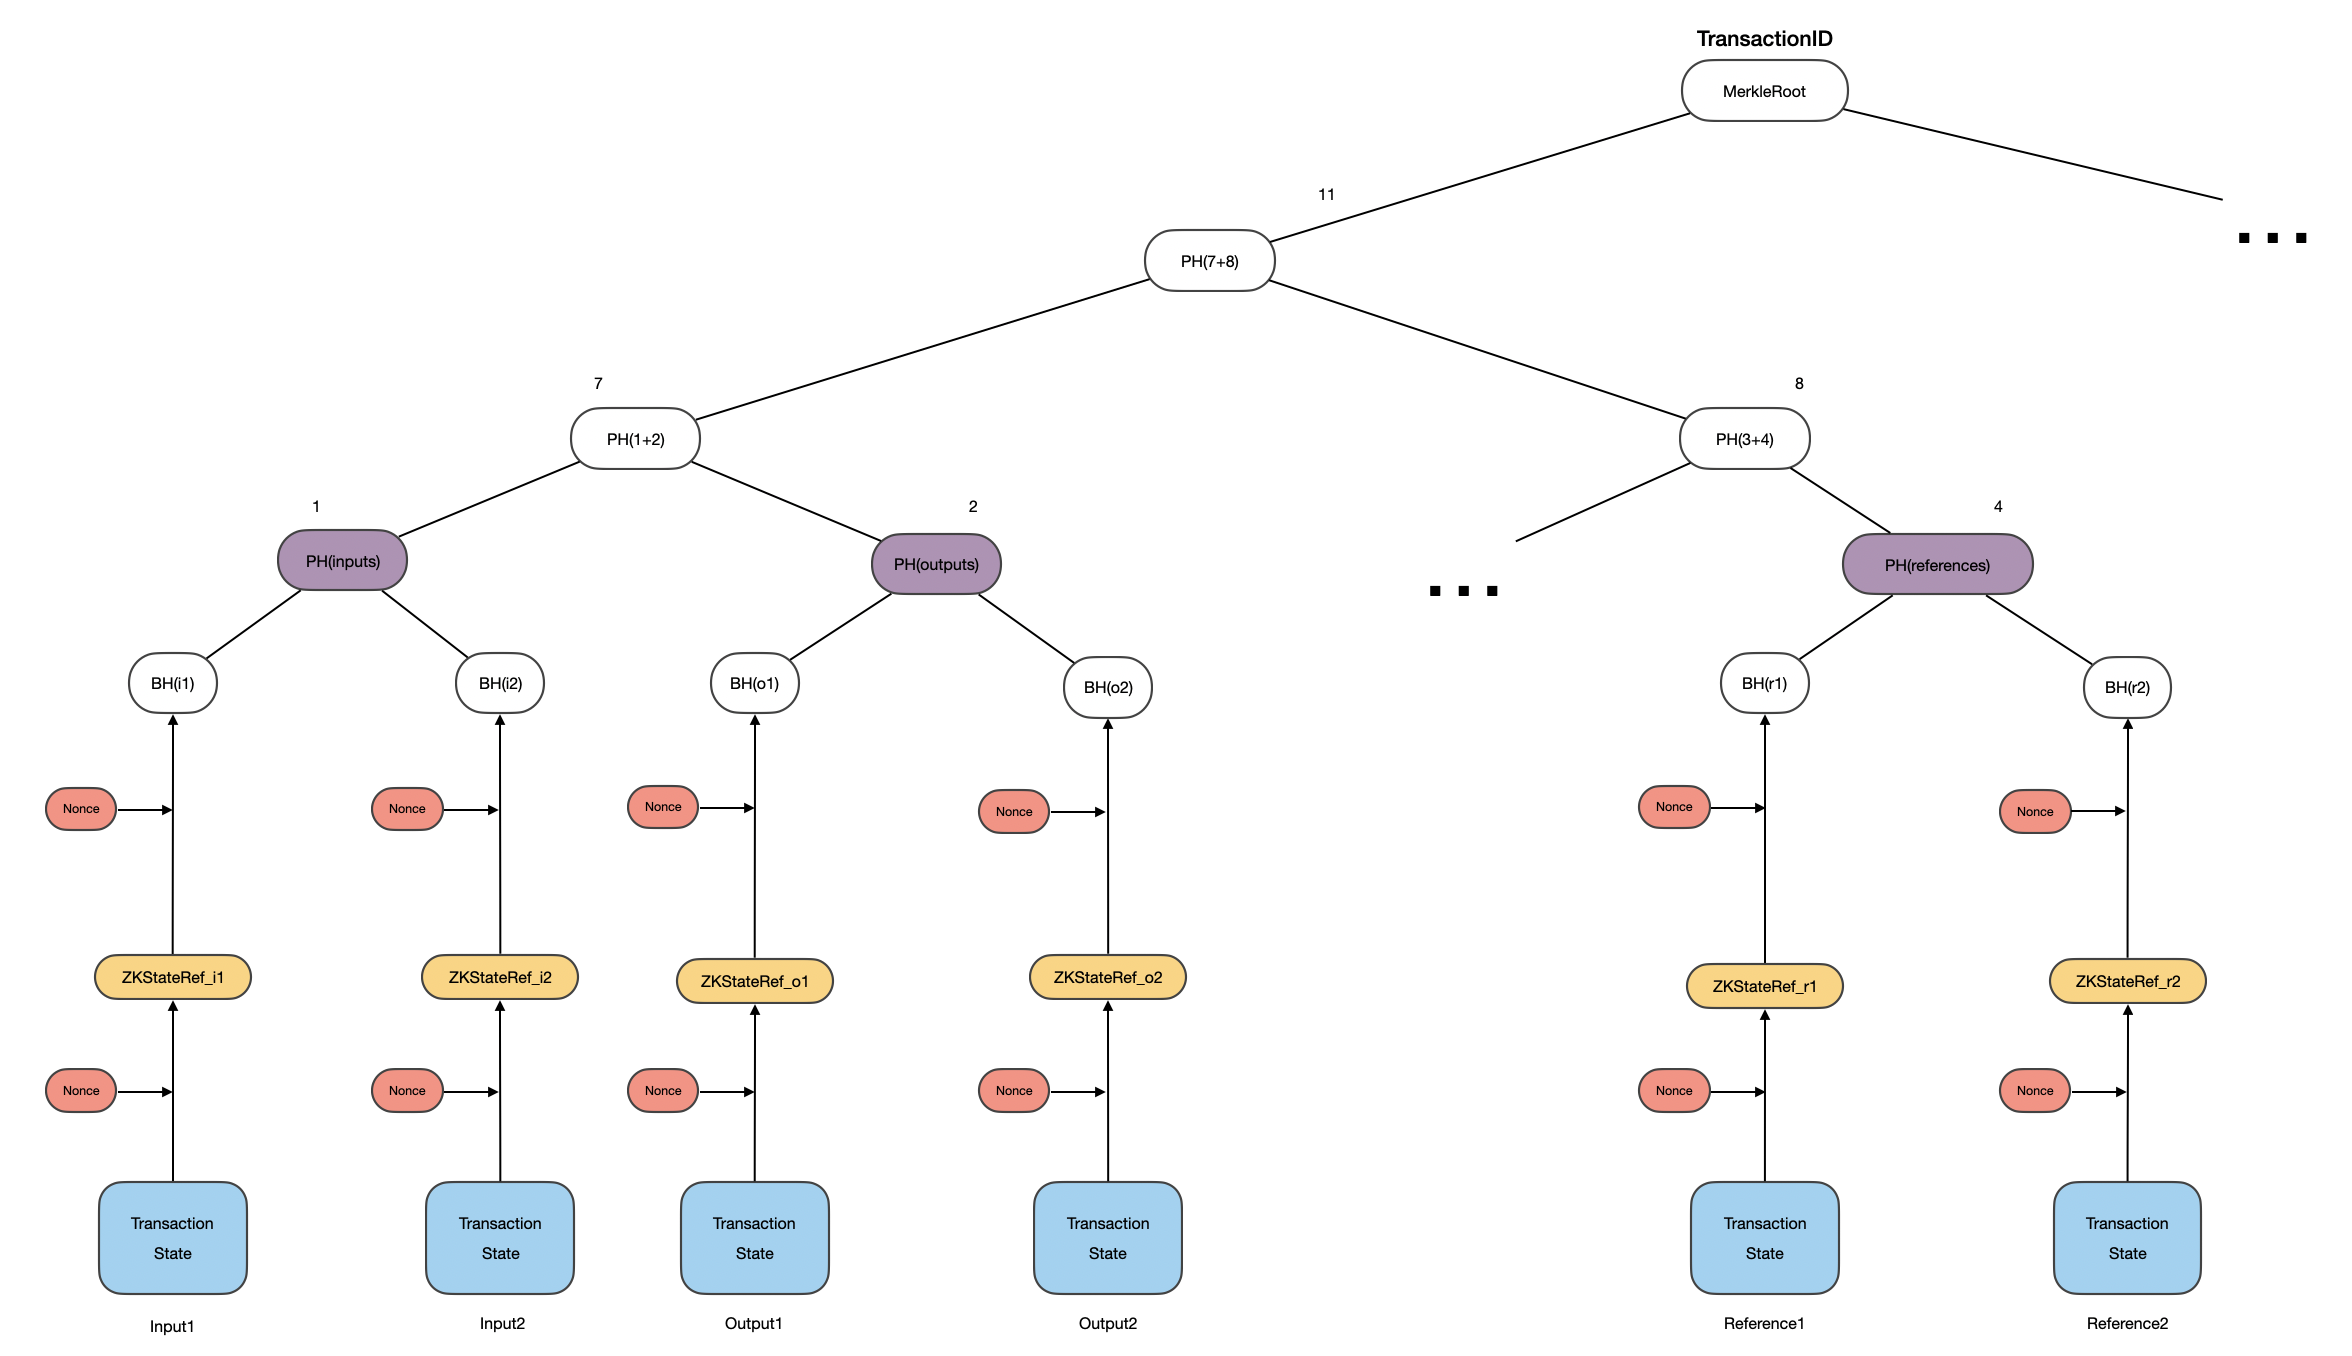
\includegraphics[width=\textwidth]{Appendix1/images/tree_ts}
\caption{Merkle Tree representation of a transaction with \texttt{Transaction State} and \texttt{ZKStateRef}.}
\label{fig:tree_ts}
\end{figure}

A \texttt{Transaction State} consists of following attributes:
\begin{itemize}
\item \texttt{data},
\item \texttt{contract},
\item \texttt{notary},
\item \texttt{encumbrance},
\item \texttt{constraint}
\end{itemize}

We can compute ZKStateRef as
\begin{align}
ZKStateRef &= Hash(nonce \concat state\_fields), \text{ s.t.} \\
state\_fields &= data \concat contract \concat notary \concat encumbrance \concat constraint \nonumber
\end{align}
\noindent and the leaf hash as
\begin{align}
LeafHash &= Hash(nonce \concat ZKStateRef).
\end{align}

Now, considering that the nonce used in the computation of ZKStateRef and LeafHash is the same, the question that we need to answer is that can a malicious party obtain meaningful information about the \texttt{Transaction State} given the public values ZKStateRef, LeafHash, and the computation of the LeafHash?
In this scenario, the malicious party (which is notary in our case) is asked to validate LeafHash by repeating the computation $LeafHash = Hash(nonce || ZKStateRef)$.
This is a reasonable scenario in our design, since the notary is asked to validate a filtered Merkle tree.
The filtered tree that the notary is going to validate is illustrated in Figure~\ref{fig:filtered_tree_ts}.

\begin{figure}[ht]
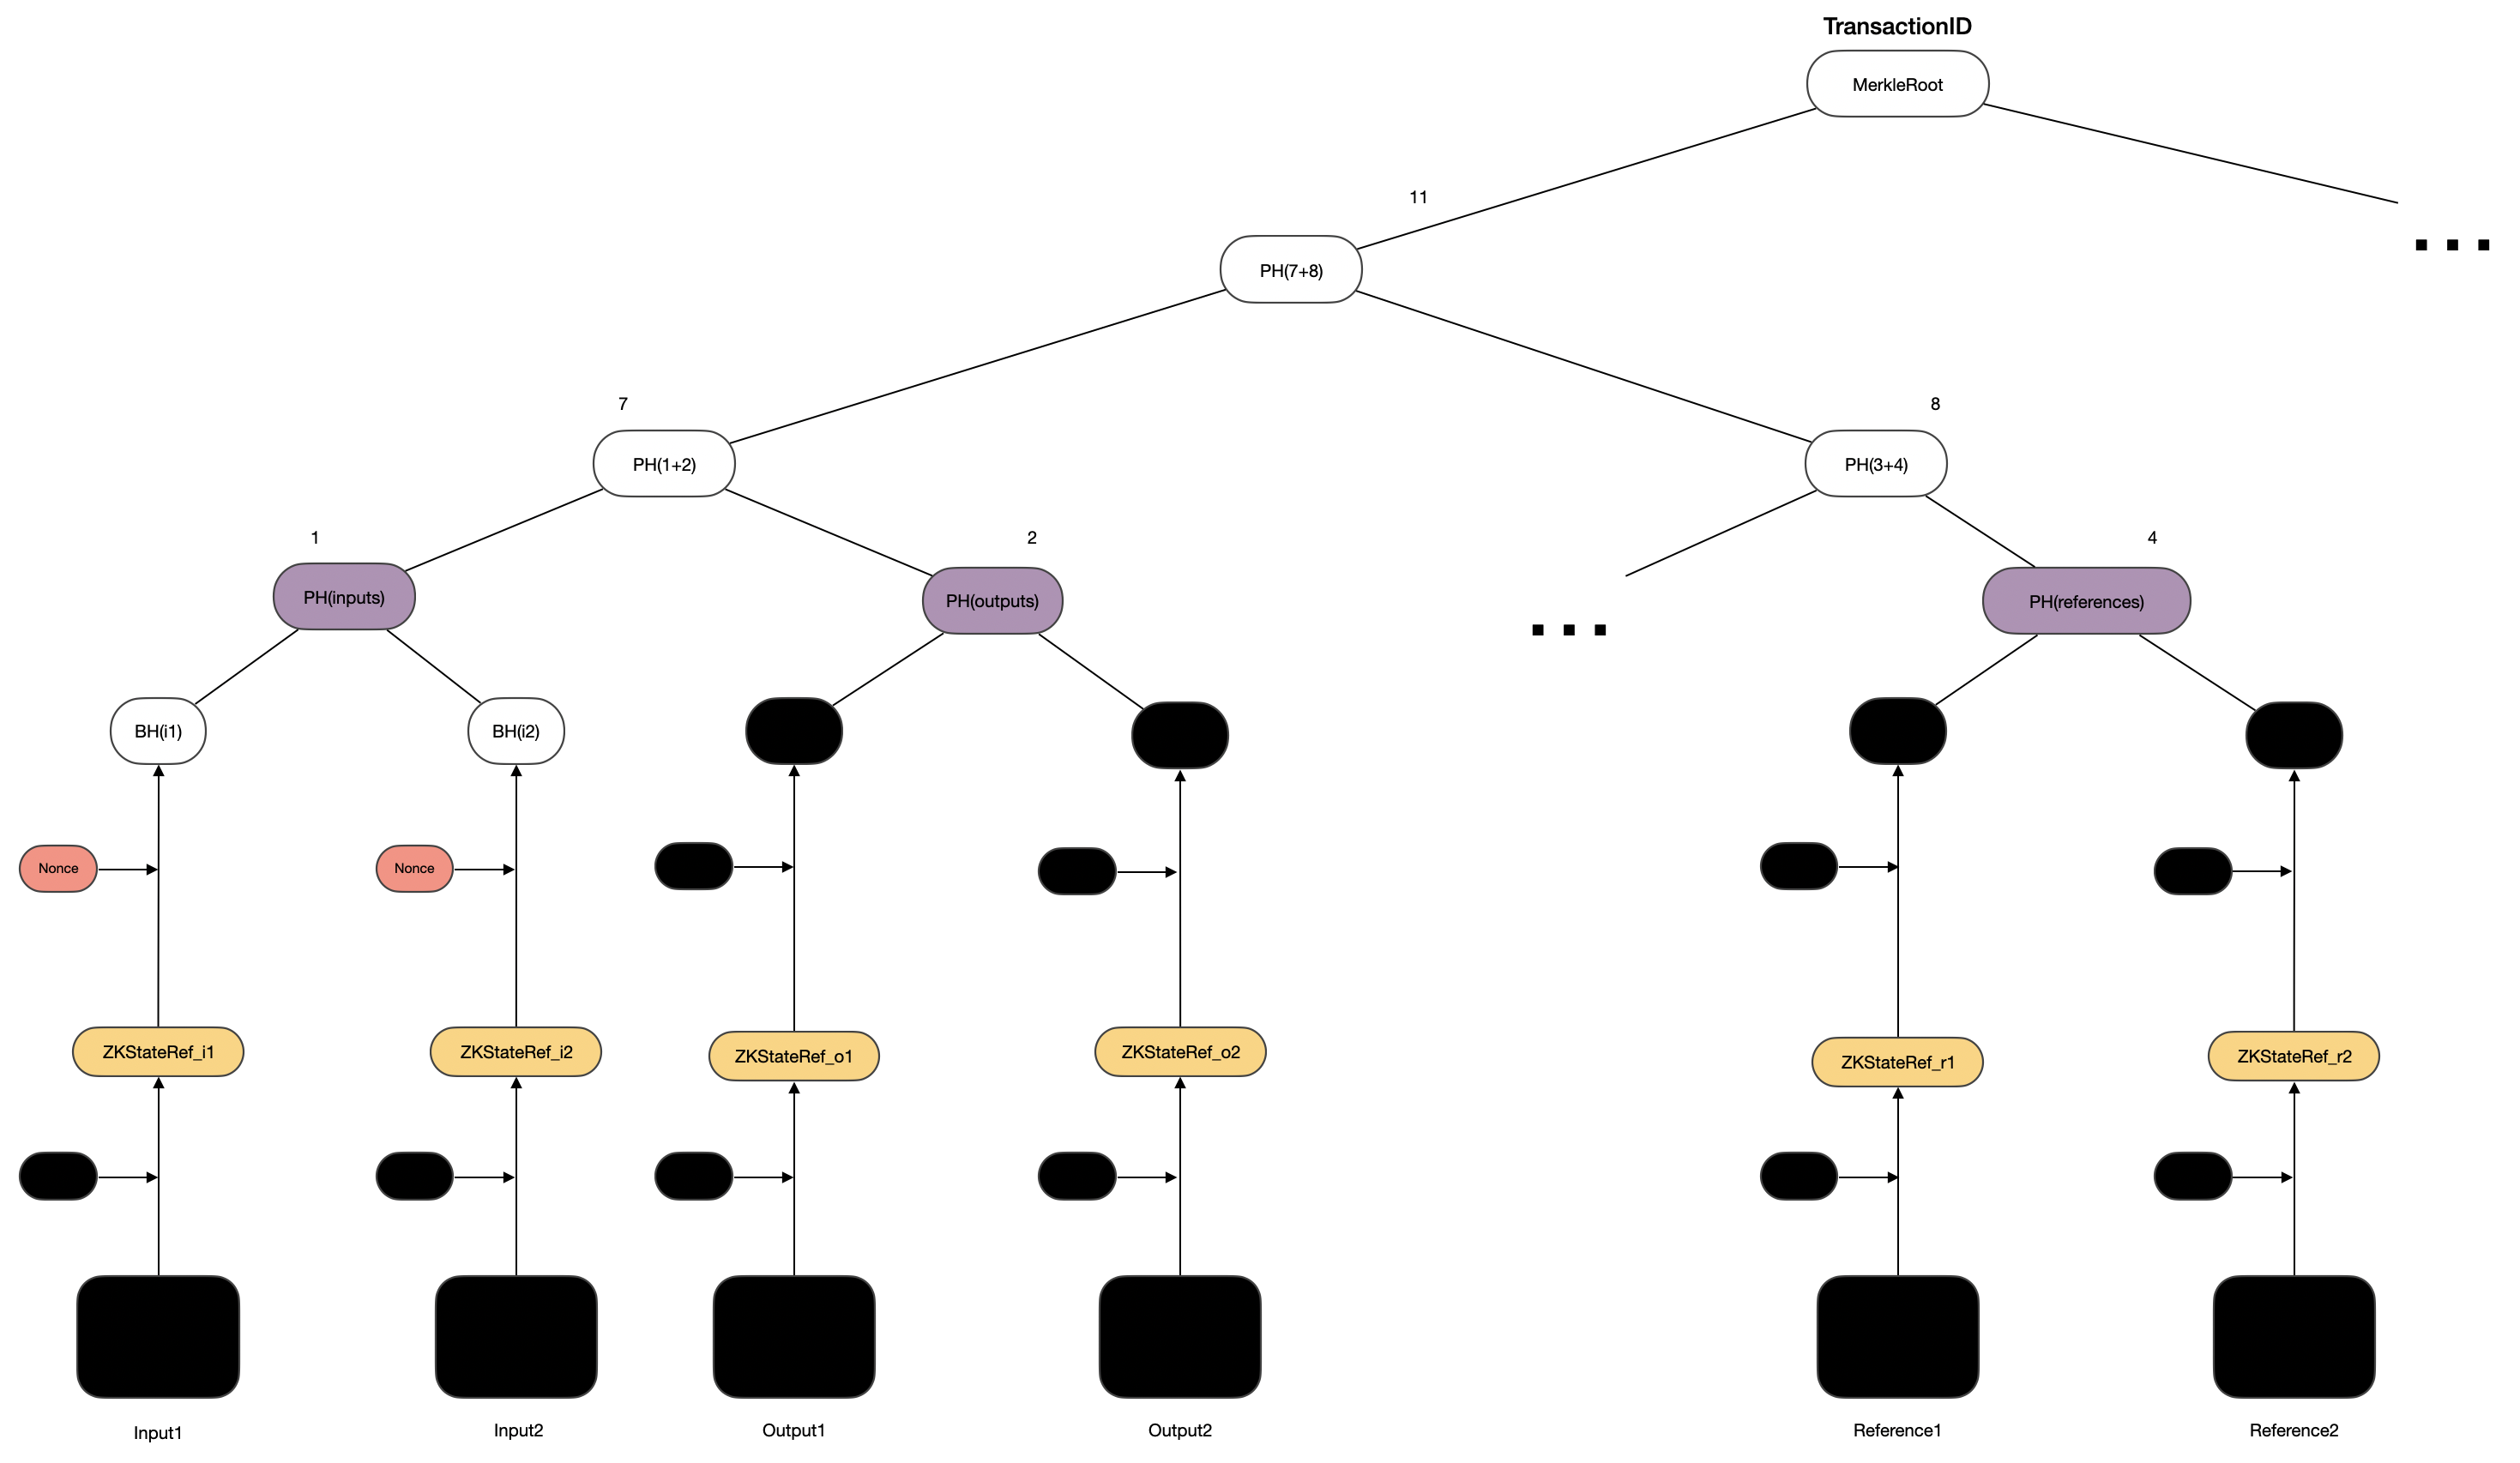
\includegraphics[width=\textwidth]{Appendix1/images/filtered_tree_ts}
\caption{Filtered Merkle Tree representation of a transaction that is validated by the notary.}
\label{fig:filtered_tree_ts}
\end{figure}

In such a scenario, the notary has access to LeafHash, nonce, and ZKStateRef.
Knowing nonce, the difficulty of applying a pre-image attack on $ZKStateRef = Hash(nonce || state\_fields)$ depends on the attacker knowing the contract logic and State object structure (which they will, because they need to know which ZKP circuit to use, so they know the contract).
Knowing the structure, they can make reasonable/educated guesses on the field values of the state based on the contract business logic.

Then, the next question is how can we compute a unique nonce for ZKStateRef without incurring too much additional cost.
We consider three options for that:

\begin{enumerate}
\item Change the order in the computation of nonce such that:
\begin{align}
LeafHash\_nonce &= Hash(privacySalt \concat groupIndex \concat elementIndex) \\
ZKStateRef\_nonce &= Hash(groupIndex \concat elementIndex \concat privacySalt)
\end{align}
\item Use the un-hashed version of nonce in the computation of ZKStateRef (it will be in the proof circuit and won't be revealed any way)
\begin{align}
ZKStateRef\_nonce = privacySalt \concat groupIndex \concat elementIndex
\end{align}
\end{enumerate}

\includesvg[width=\textwidth]{Appendix1/images/fig1}

Some more info. And more.























\chapter*{Design Choices}

\subsection{Transaction representation:Merkle Tree vs Concatenation}

\subsection{Selection of Nonce for ZKStateRef}

\textbf{Problem:} ZKStateRef can be computed as $\text{ZKStateRef} = Hash(\text{Transaction State})$.
However, this computation is not resistant to pre-image attacks and collisions.

A solution to this problem is adding a nonce in computation such that $\text{ZKStateRef} = Hash(\text{nonce} \concat \text{Transaction State})$, which can prevent such attacks.
However, generating a nonce in Corda requires to perform a hash operation which is a costly operation in ZK circuits.
As an alternative, \textit{can we use the same nonce that is generated for the hashing of component elements?}

Before answering this question, we provide some information about the data that is used in the computation of ZKStateRef.
We compute ZKStateRef for input, output, and reference components.
Each element in these component groups are a \texttt{ZKStateAndRef} object which consists of a \texttt{Transaction State} and \texttt{ZKStateRef}.
Figure~\ref{fig:tree_ts} shows the relation between each object.

\begin{figure}[ht]
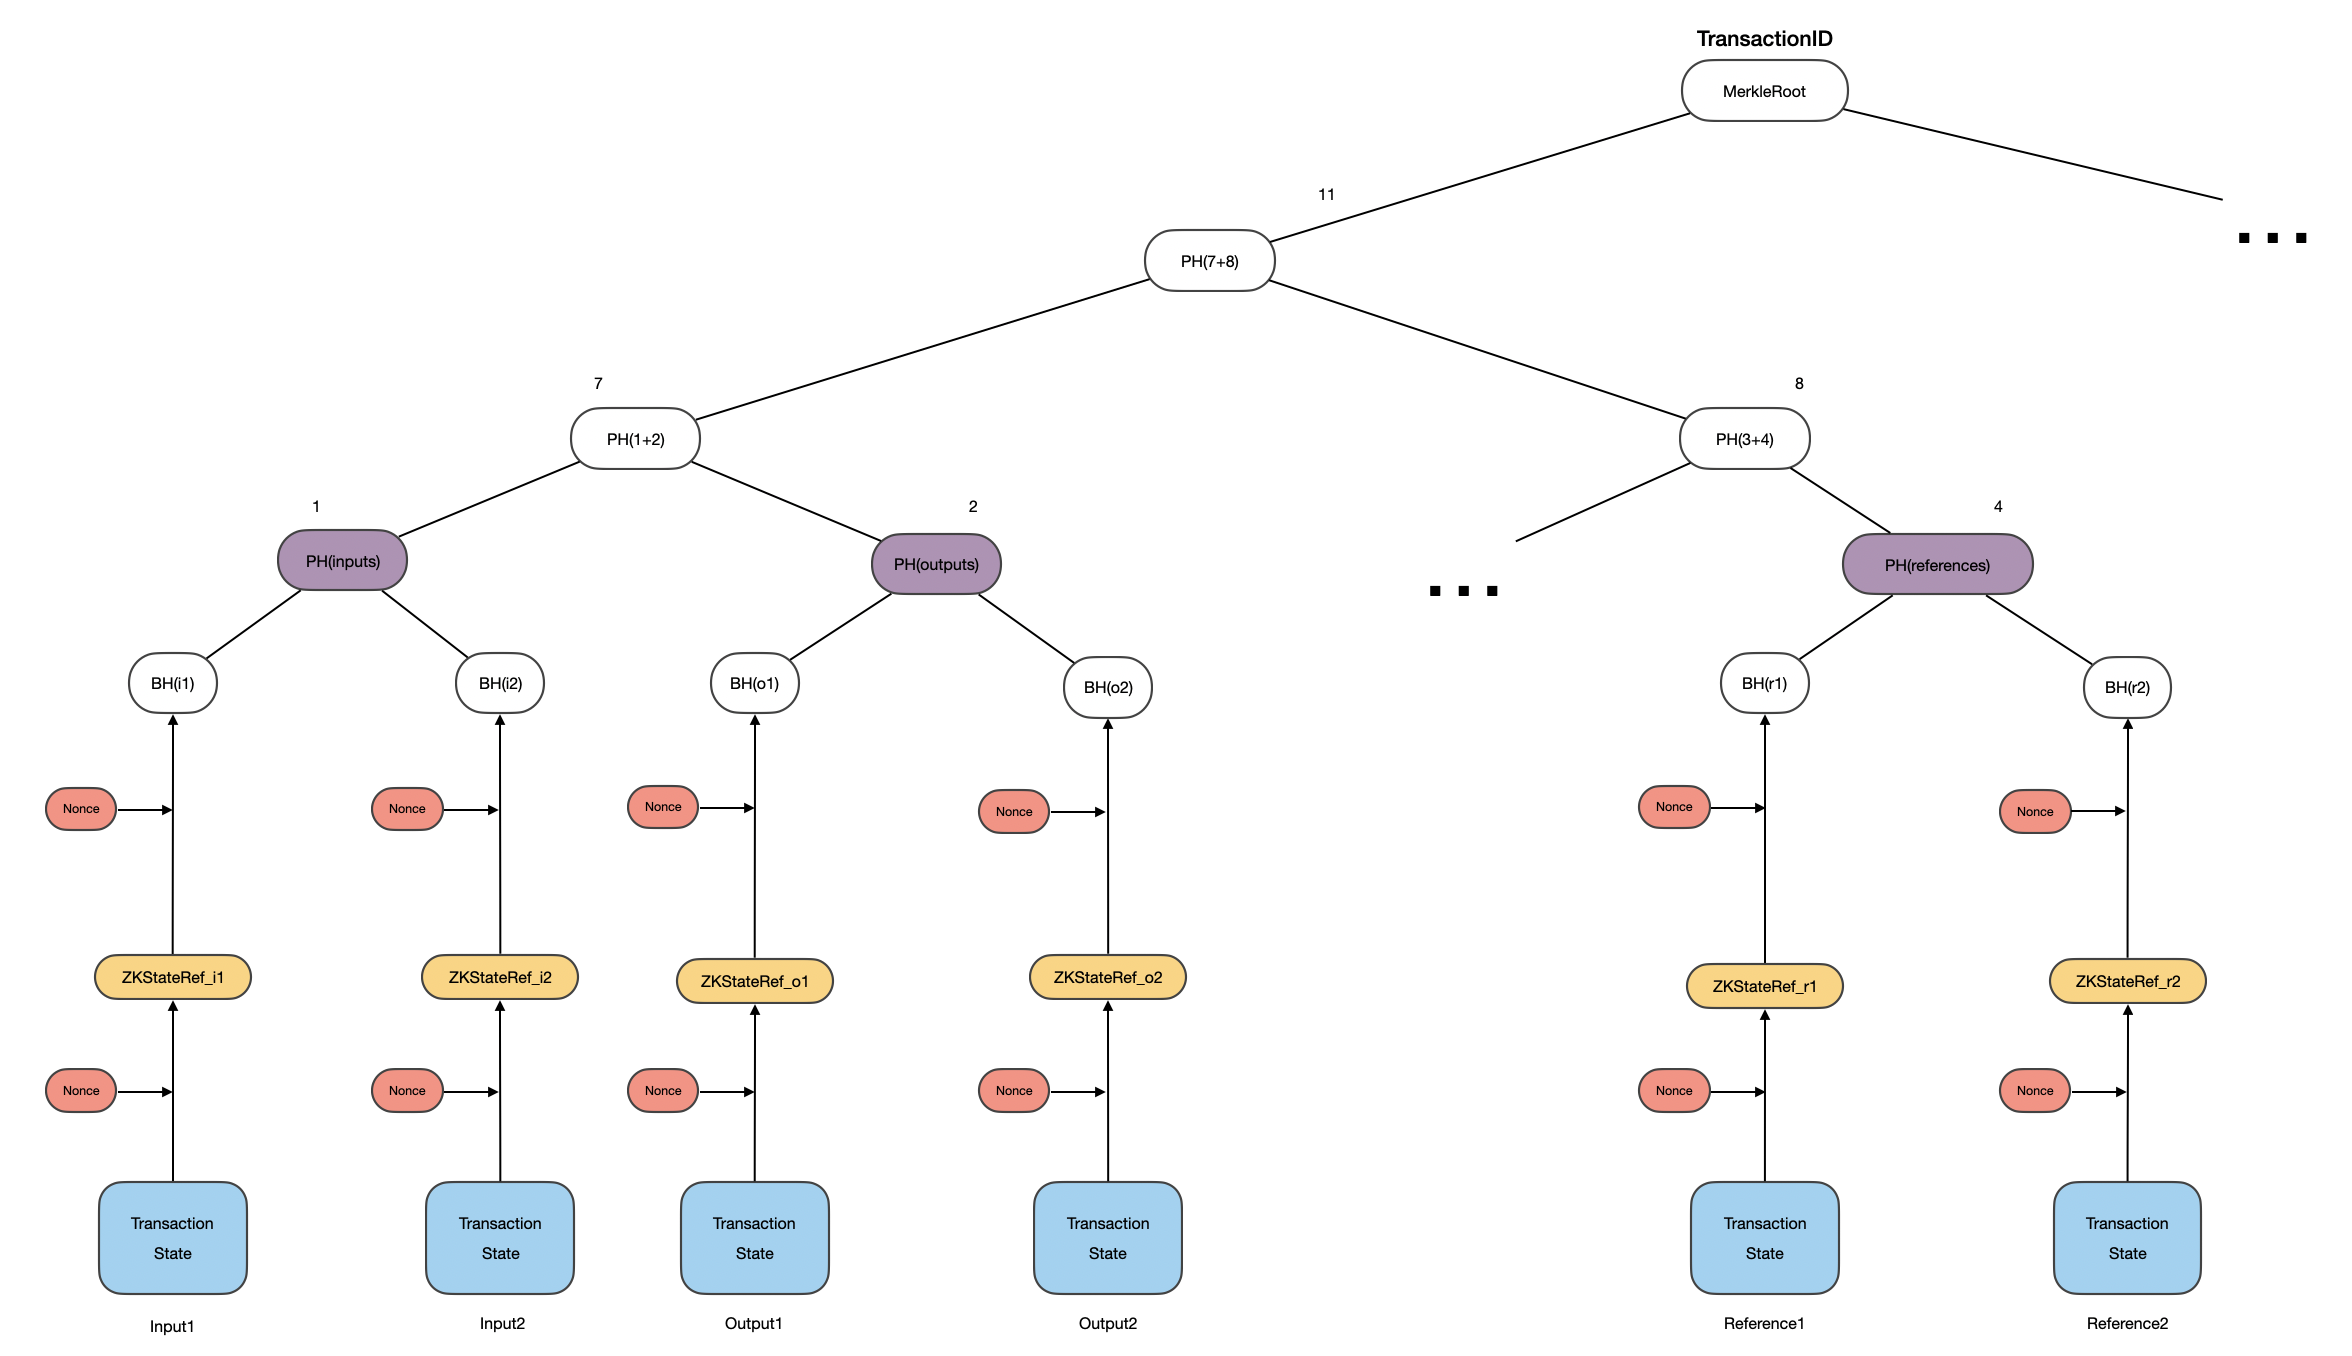
\includegraphics[width=\textwidth]{Appendix1/images/tree_ts}
\caption{Merkle Tree representation of a transaction with \texttt{Transaction State} and \texttt{ZKStateRef}.}
\label{fig:tree_ts}
\end{figure}

A \texttt{Transaction State} consists of following attributes:
\begin{itemize}
\item \texttt{data},
\item \texttt{contract},
\item \texttt{notary},
\item \texttt{encumbrance},
\item \texttt{constraint}
\end{itemize}

We can compute ZKStateRef as
\begin{align}
ZKStateRef &= Hash(nonce \concat state\_fields), \text{ s.t.} \\
state\_fields &= data \concat contract \concat notary \concat encumbrance \concat constraint \nonumber
\end{align}
\noindent and the leaf hash as
\begin{align}
LeafHash &= Hash(nonce \concat ZKStateRef).
\end{align}

Now, considering that the nonce used in the computation of ZKStateRef and LeafHash is the same, the question that we need to answer is that can a malicious party obtain meaningful information about the \texttt{Transaction State} given the public values ZKStateRef, LeafHash, and the computation of the LeafHash?
In this scenario, the malicious party (which is notary in our case) is asked to validate LeafHash by repeating the computation $LeafHash = Hash(nonce || ZKStateRef)$.
This is a reasonable scenario in our design, since the notary is asked to validate a filtered Merkle tree.
The filtered tree that the notary is going to validate is illustrated in Figure~\ref{fig:filtered_tree_ts}.

\begin{figure}[ht]
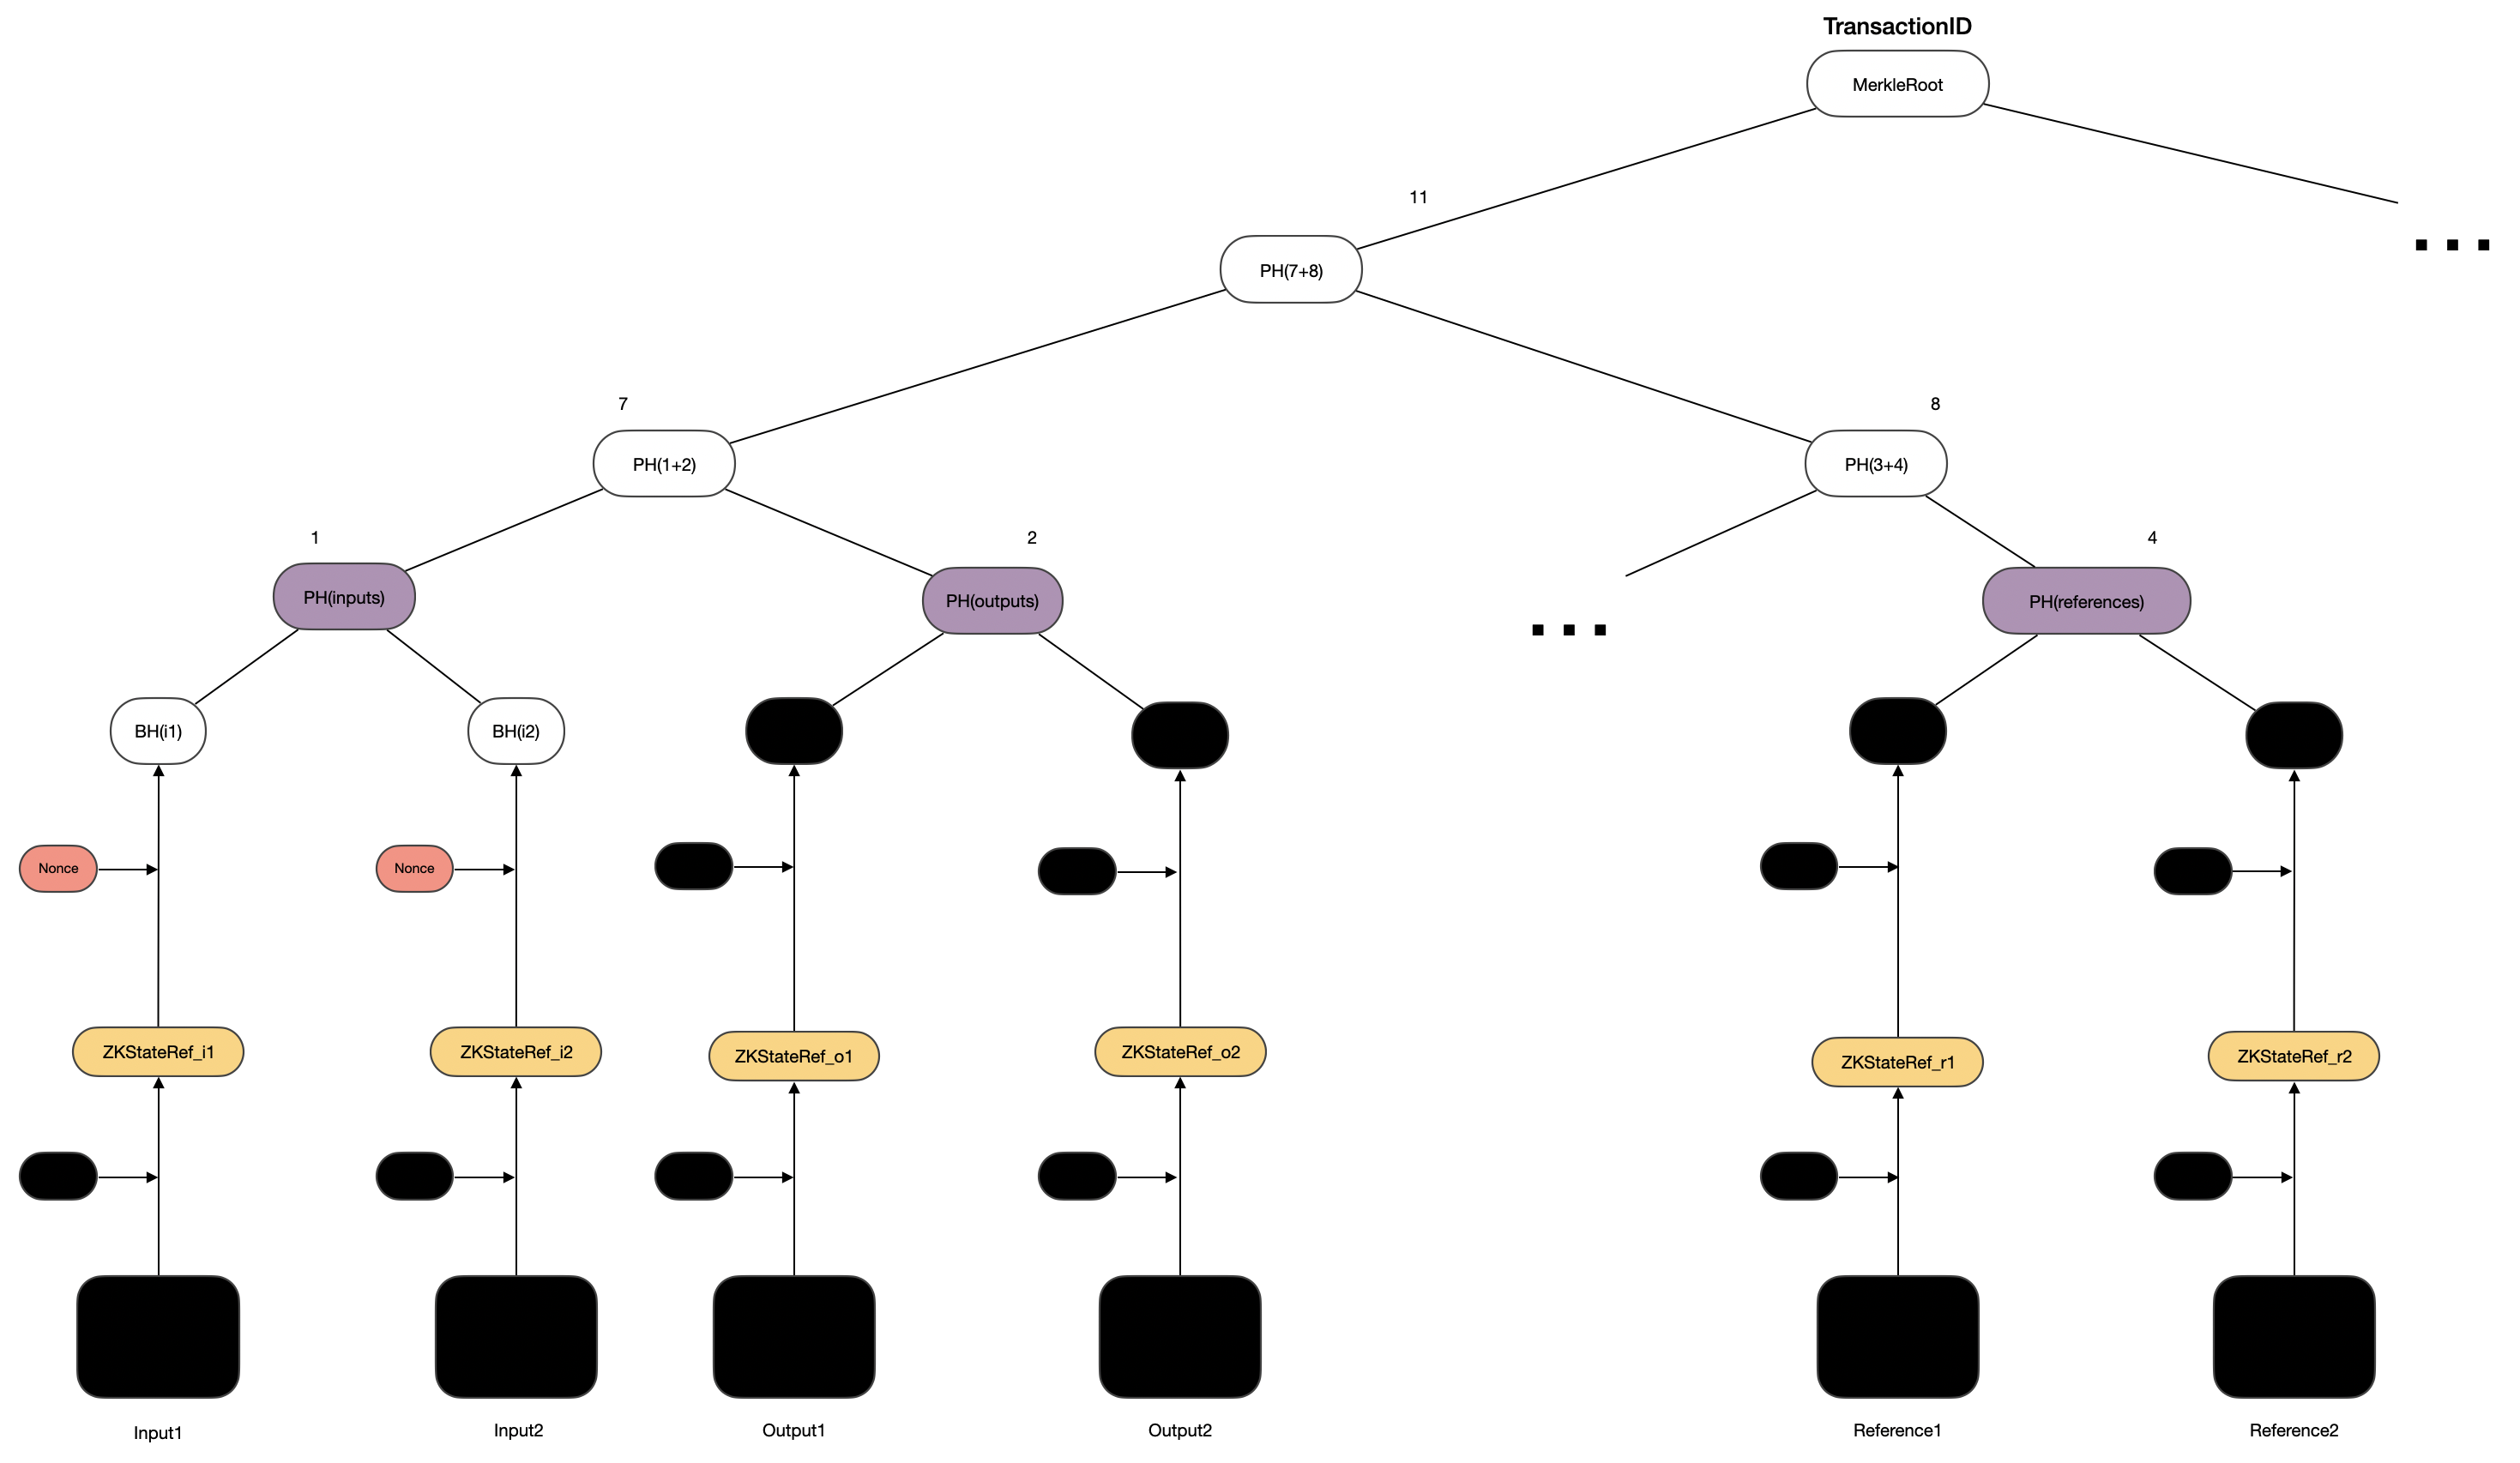
\includegraphics[width=\textwidth]{Appendix1/images/filtered_tree_ts}
\caption{Filtered Merkle Tree representation of a transaction that is validated by the notary.}
\label{fig:filtered_tree_ts}
\end{figure}

In such a scenario, the notary has access to LeafHash, nonce, and ZKStateRef.
Knowing nonce, the difficulty of applying a pre-image attack on $ZKStateRef = Hash(nonce || state\_fields)$ depends on the attacker knowing the contract logic and State object structure (which they will, because they need to know which ZKP circuit to use, so they know the contract).
Knowing the structure, they can make reasonable/educated guesses on the field values of the state based on the contract business logic.

Then, the next question is how can we compute a unique nonce for ZKStateRef without incurring too much additional cost.
We consider three options for that:

\begin{enumerate}
\item Change the order in the computation of nonce such that:
\begin{align}
LeafHash\_nonce &= Hash(privacySalt \concat groupIndex \concat elementIndex) \\
ZKStateRef\_nonce &= Hash(groupIndex \concat elementIndex \concat privacySalt)
\end{align}
\item Use the un-hashed version of nonce in the computation of ZKStateRef (it will be in the proof circuit and won't be revealed any way)
\begin{align}
ZKStateRef\_nonce = privacySalt \concat groupIndex \concat elementIndex
\end{align}
\end{enumerate}

\includesvg[width=\textwidth]{Appendix1/images/fig1}

Some more info. And more.























\chapter*{Design Choices}

\subsection{Transaction representation:Merkle Tree vs Concatenation}

\subsection{Selection of Nonce for ZKStateRef}

\textbf{Problem:} ZKStateRef can be computed as $\text{ZKStateRef} = Hash(\text{Transaction State})$.
However, this computation is not resistant to pre-image attacks and collisions.

A solution to this problem is adding a nonce in computation such that $\text{ZKStateRef} = Hash(\text{nonce} \concat \text{Transaction State})$, which can prevent such attacks.
However, generating a nonce in Corda requires to perform a hash operation which is a costly operation in ZK circuits.
As an alternative, \textit{can we use the same nonce that is generated for the hashing of component elements?}

Before answering this question, we provide some information about the data that is used in the computation of ZKStateRef.
We compute ZKStateRef for input, output, and reference components.
Each element in these component groups are a \texttt{ZKStateAndRef} object which consists of a \texttt{Transaction State} and \texttt{ZKStateRef}.
Figure~\ref{fig:tree_ts} shows the relation between each object.

\begin{figure}[ht]
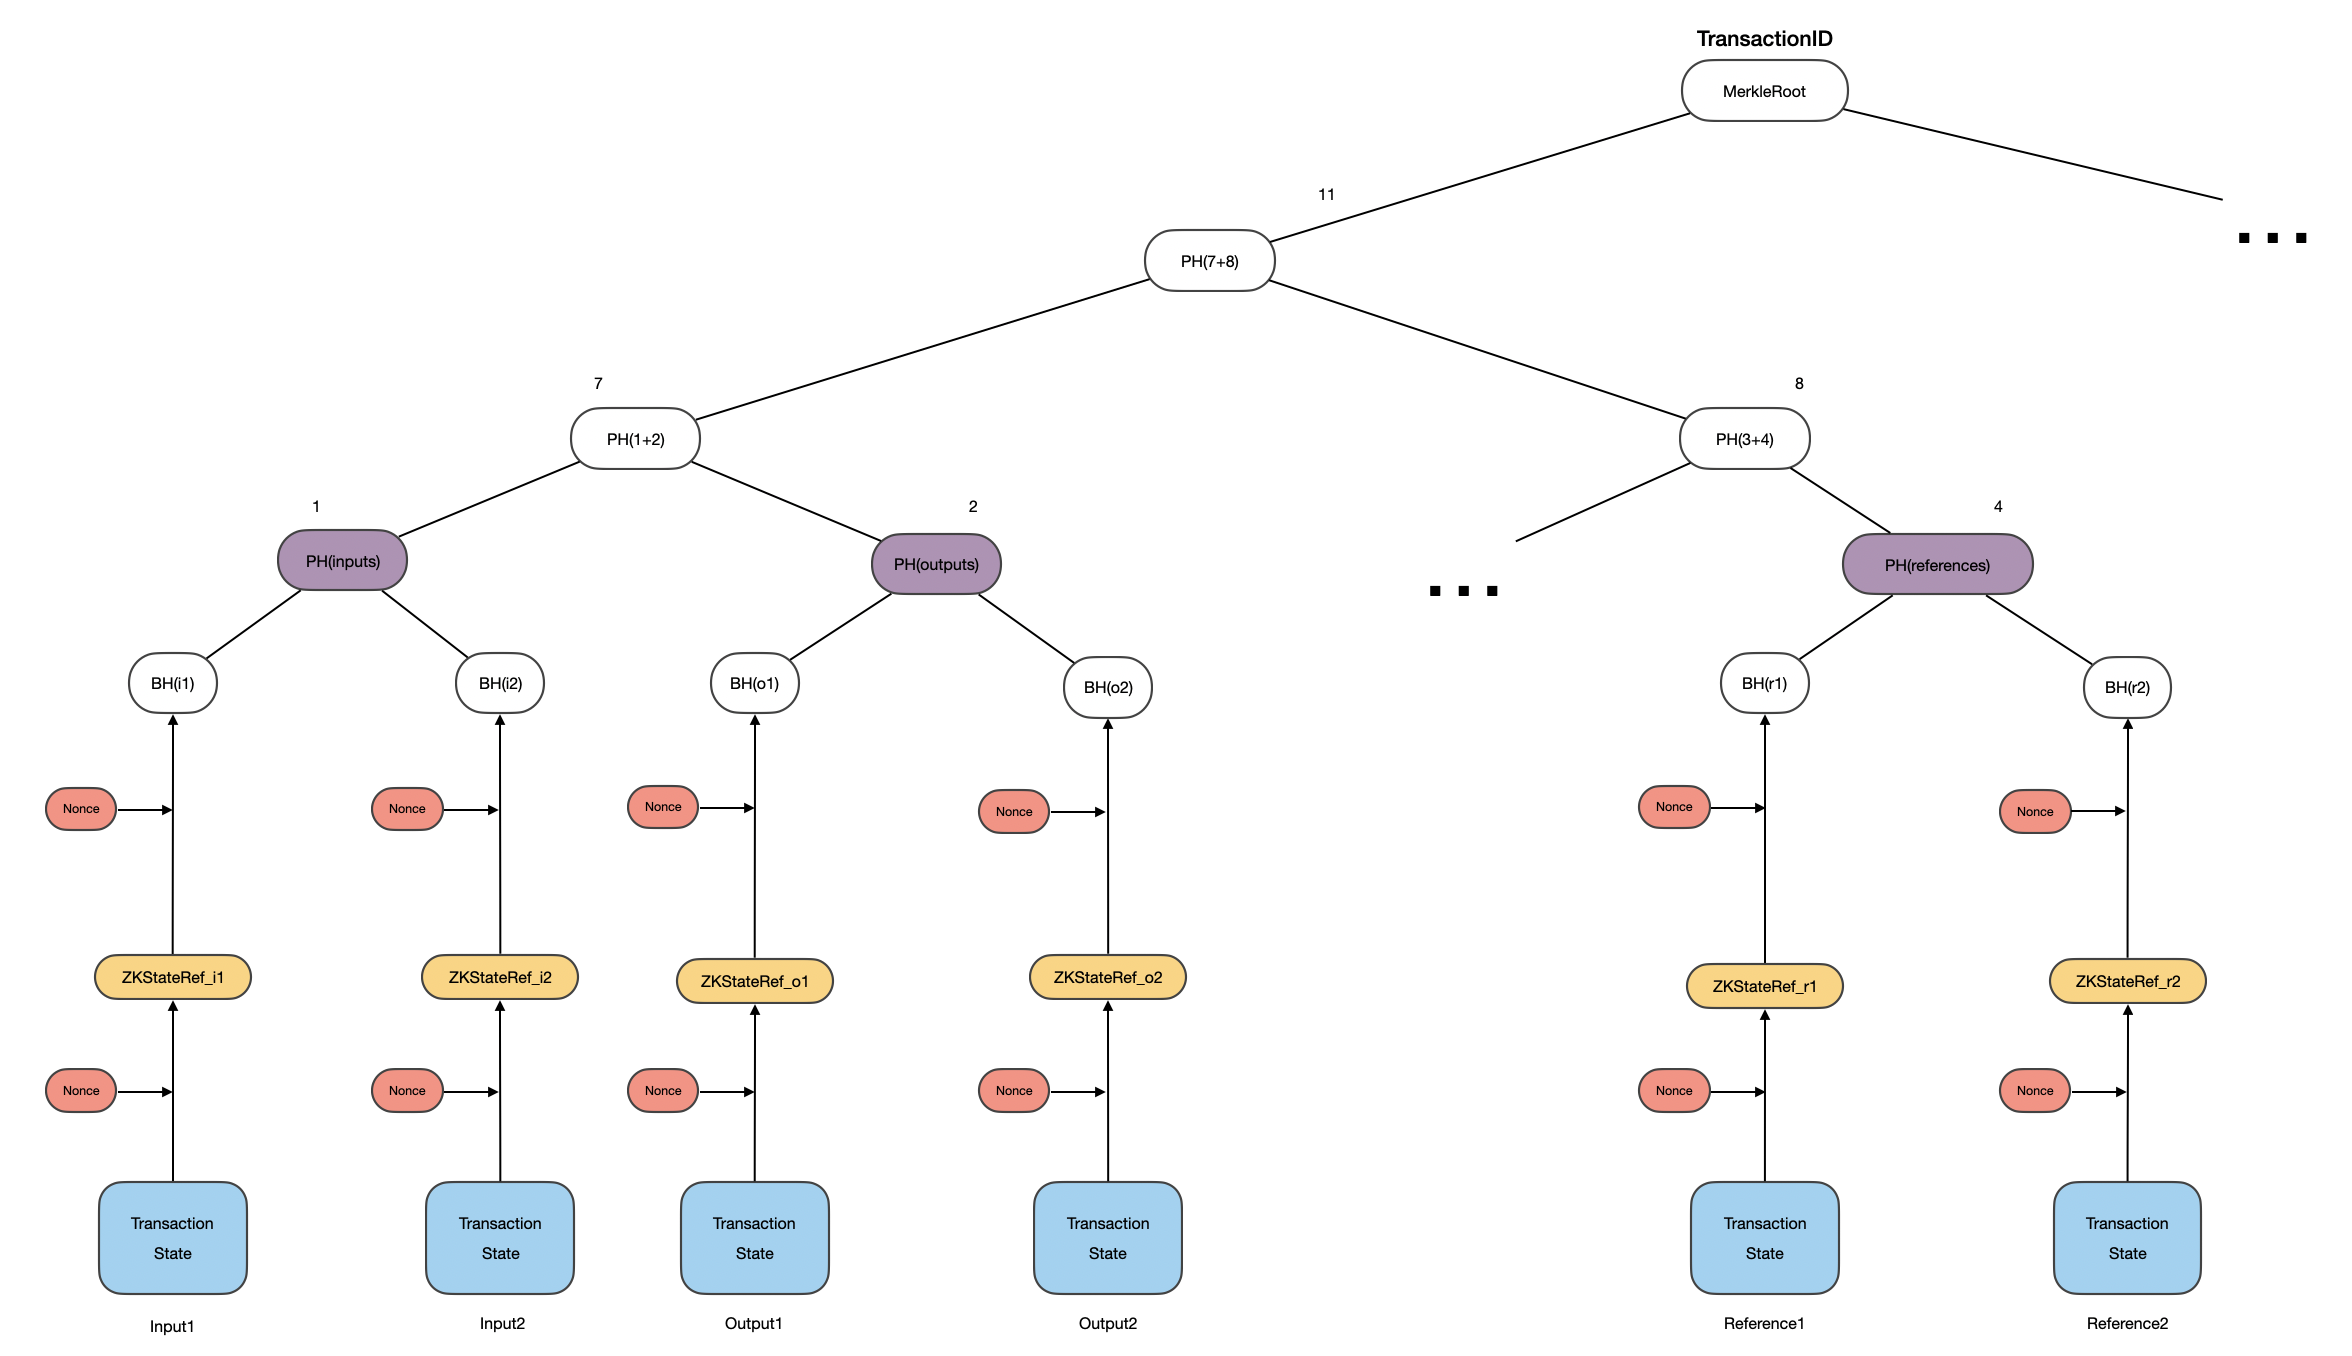
\includegraphics[width=\textwidth]{Appendix1/images/tree_ts}
\caption{Merkle Tree representation of a transaction with \texttt{Transaction State} and \texttt{ZKStateRef}.}
\label{fig:tree_ts}
\end{figure}

A \texttt{Transaction State} consists of following attributes:
\begin{itemize}
\item \texttt{data},
\item \texttt{contract},
\item \texttt{notary},
\item \texttt{encumbrance},
\item \texttt{constraint}
\end{itemize}

We can compute ZKStateRef as
\begin{align}
ZKStateRef &= Hash(nonce \concat state\_fields), \text{ s.t.} \\
state\_fields &= data \concat contract \concat notary \concat encumbrance \concat constraint \nonumber
\end{align}
\noindent and the leaf hash as
\begin{align}
LeafHash &= Hash(nonce \concat ZKStateRef).
\end{align}

Now, considering that the nonce used in the computation of ZKStateRef and LeafHash is the same, the question that we need to answer is that can a malicious party obtain meaningful information about the \texttt{Transaction State} given the public values ZKStateRef, LeafHash, and the computation of the LeafHash?
In this scenario, the malicious party (which is notary in our case) is asked to validate LeafHash by repeating the computation $LeafHash = Hash(nonce || ZKStateRef)$.
This is a reasonable scenario in our design, since the notary is asked to validate a filtered Merkle tree.
The filtered tree that the notary is going to validate is illustrated in Figure~\ref{fig:filtered_tree_ts}.

\begin{figure}[ht]
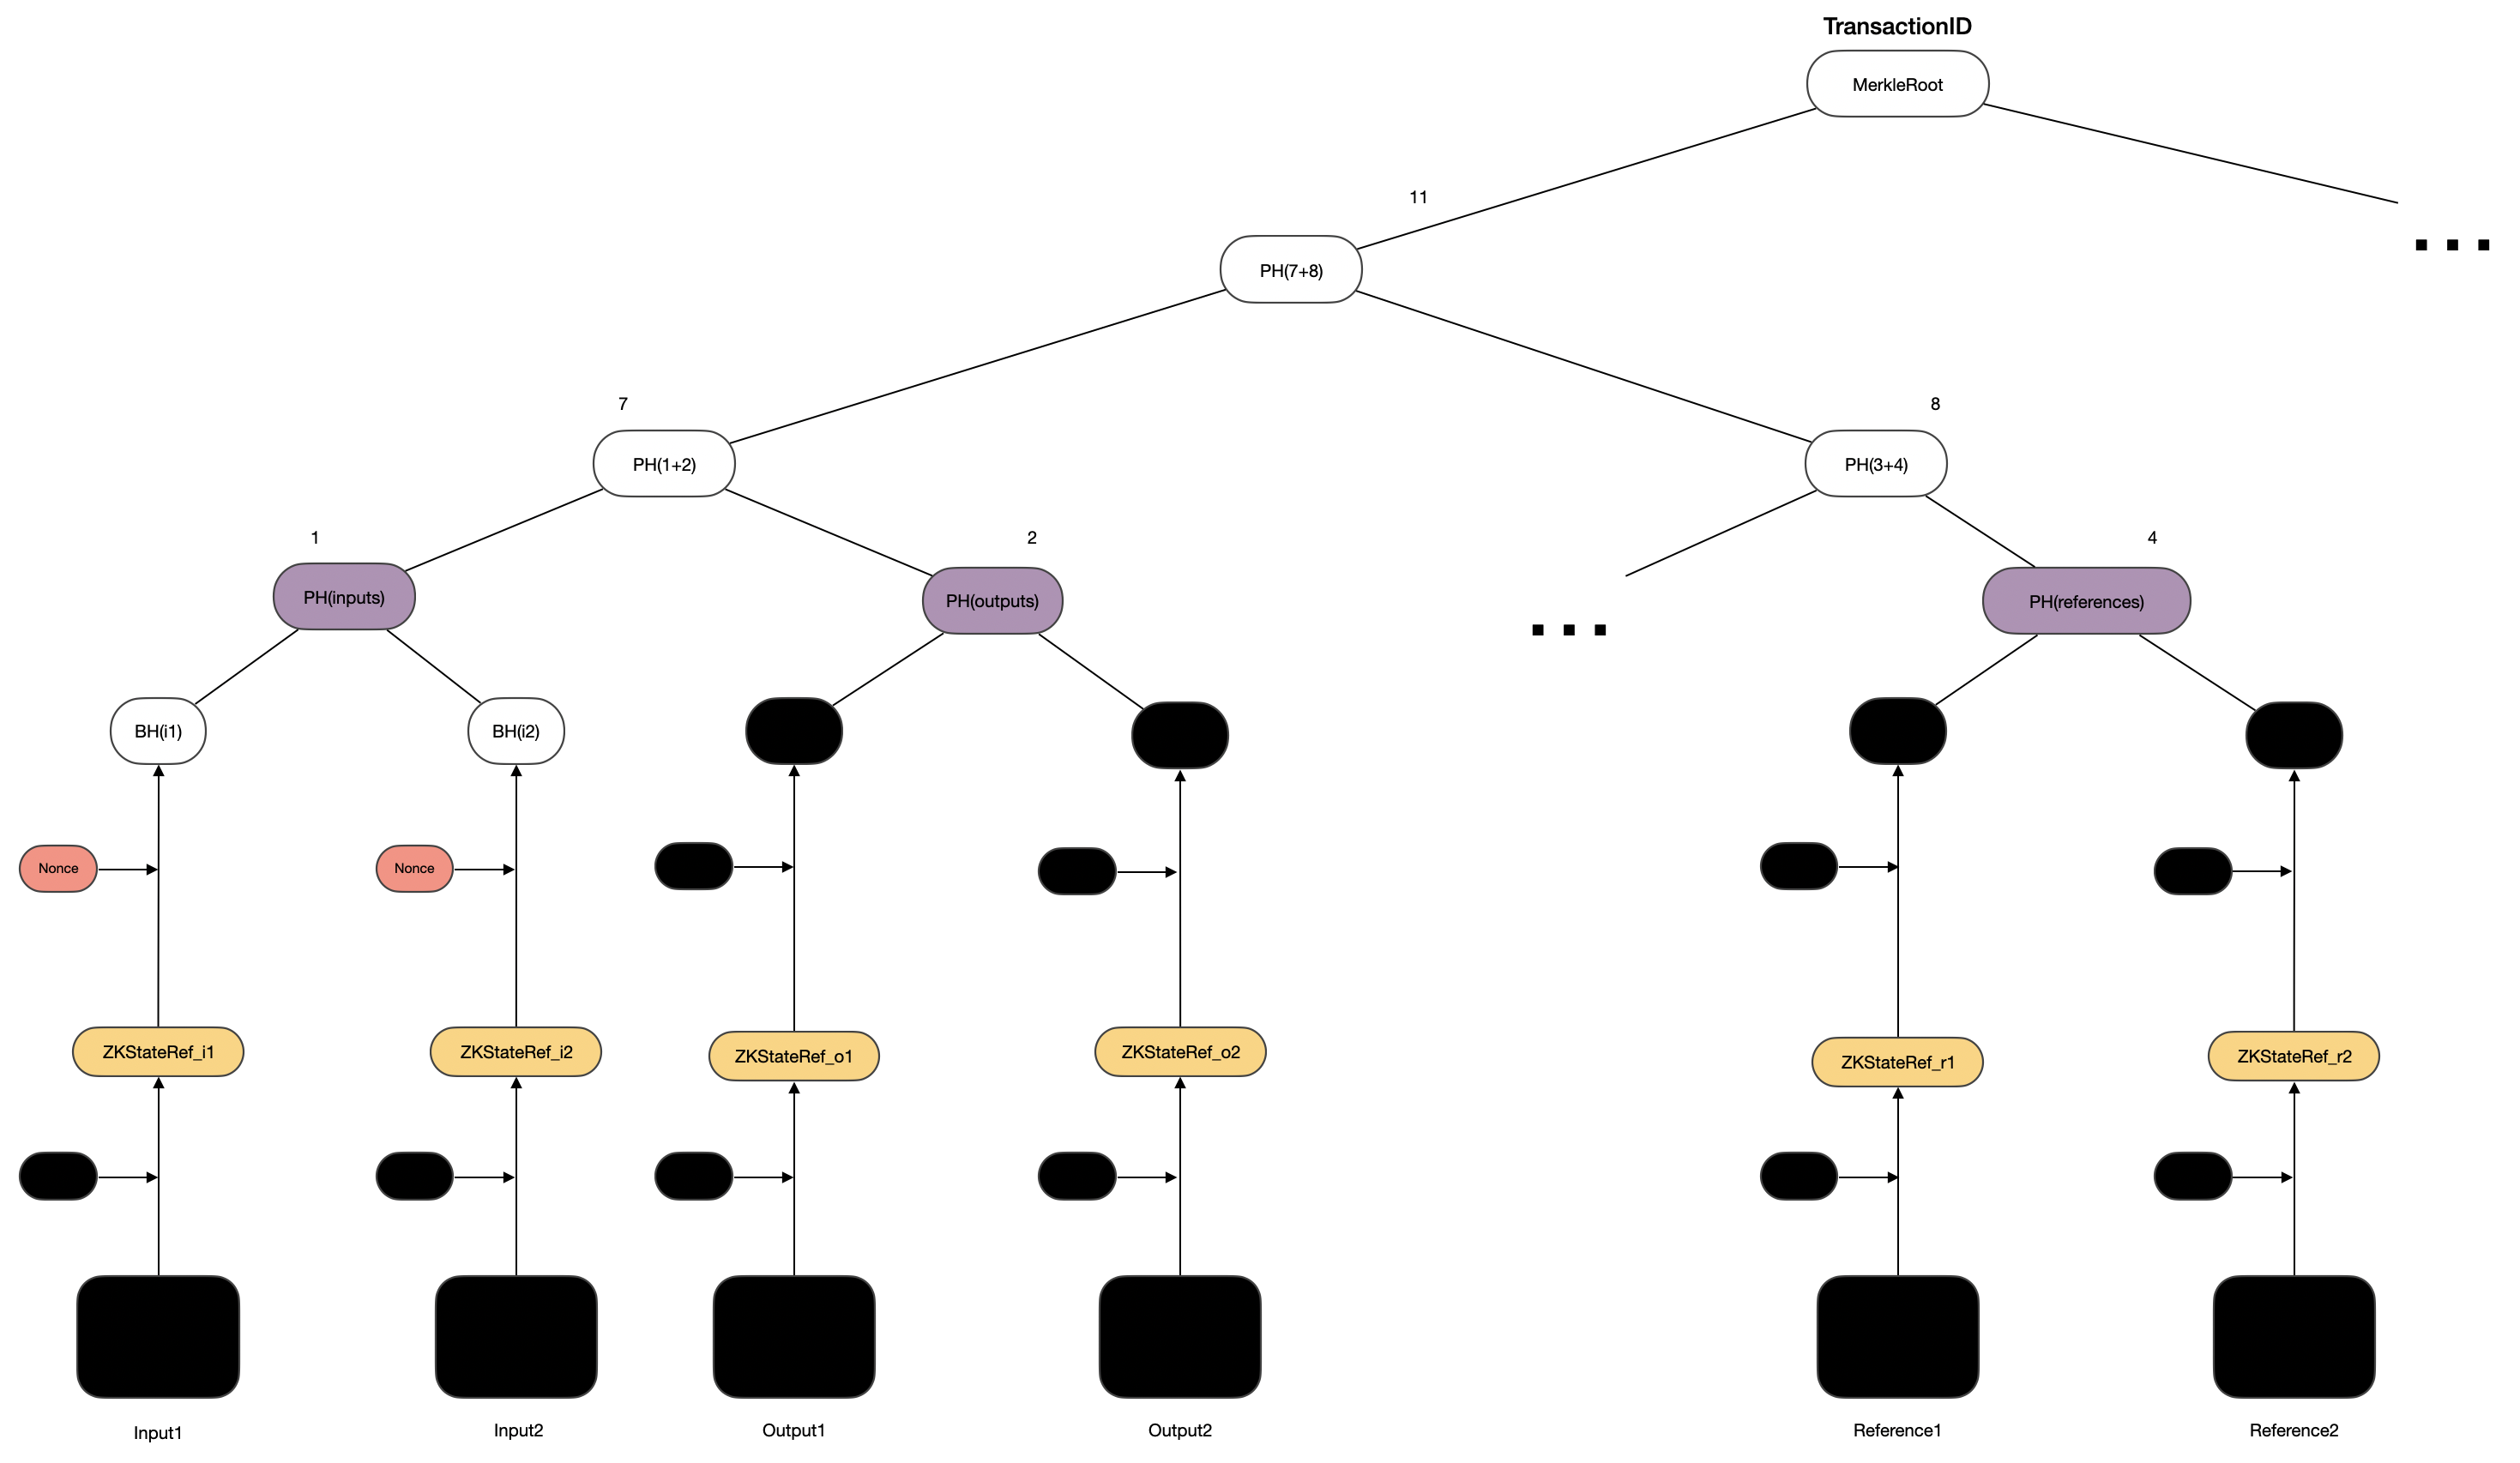
\includegraphics[width=\textwidth]{Appendix1/images/filtered_tree_ts}
\caption{Filtered Merkle Tree representation of a transaction that is validated by the notary.}
\label{fig:filtered_tree_ts}
\end{figure}

In such a scenario, the notary has access to LeafHash, nonce, and ZKStateRef.
Knowing nonce, the difficulty of applying a pre-image attack on $ZKStateRef = Hash(nonce || state\_fields)$ depends on the attacker knowing the contract logic and State object structure (which they will, because they need to know which ZKP circuit to use, so they know the contract).
Knowing the structure, they can make reasonable/educated guesses on the field values of the state based on the contract business logic.

Then, the next question is how can we compute a unique nonce for ZKStateRef without incurring too much additional cost.
We consider three options for that:

\begin{enumerate}
\item Change the order in the computation of nonce such that:
\begin{align}
LeafHash\_nonce &= Hash(privacySalt \concat groupIndex \concat elementIndex) \\
ZKStateRef\_nonce &= Hash(groupIndex \concat elementIndex \concat privacySalt)
\end{align}
\item Use the un-hashed version of nonce in the computation of ZKStateRef (it will be in the proof circuit and won't be revealed any way)
\begin{align}
ZKStateRef\_nonce = privacySalt \concat groupIndex \concat elementIndex
\end{align}
\end{enumerate}

\includesvg[width=\textwidth]{Appendix1/images/fig1}

Some more info. And more.























\chapter*{Design Choices}

\subsection{Transaction representation:Merkle Tree vs Concatenation}

\subsection{Selection of Nonce for ZKStateRef}

\textbf{Problem:} ZKStateRef can be computed as $\text{ZKStateRef} = Hash(\text{Transaction State})$.
However, this computation is not resistant to pre-image attacks and collisions.

A solution to this problem is adding a nonce in computation such that $\text{ZKStateRef} = Hash(\text{nonce} \concat \text{Transaction State})$, which can prevent such attacks.
However, generating a nonce in Corda requires to perform a hash operation which is a costly operation in ZK circuits.
As an alternative, \textit{can we use the same nonce that is generated for the hashing of component elements?}

Before answering this question, we provide some information about the data that is used in the computation of ZKStateRef.
We compute ZKStateRef for input, output, and reference components.
Each element in these component groups are a \texttt{ZKStateAndRef} object which consists of a \texttt{Transaction State} and \texttt{ZKStateRef}.
Figure~\ref{fig:tree_ts} shows the relation between each object.

\begin{figure}[ht]
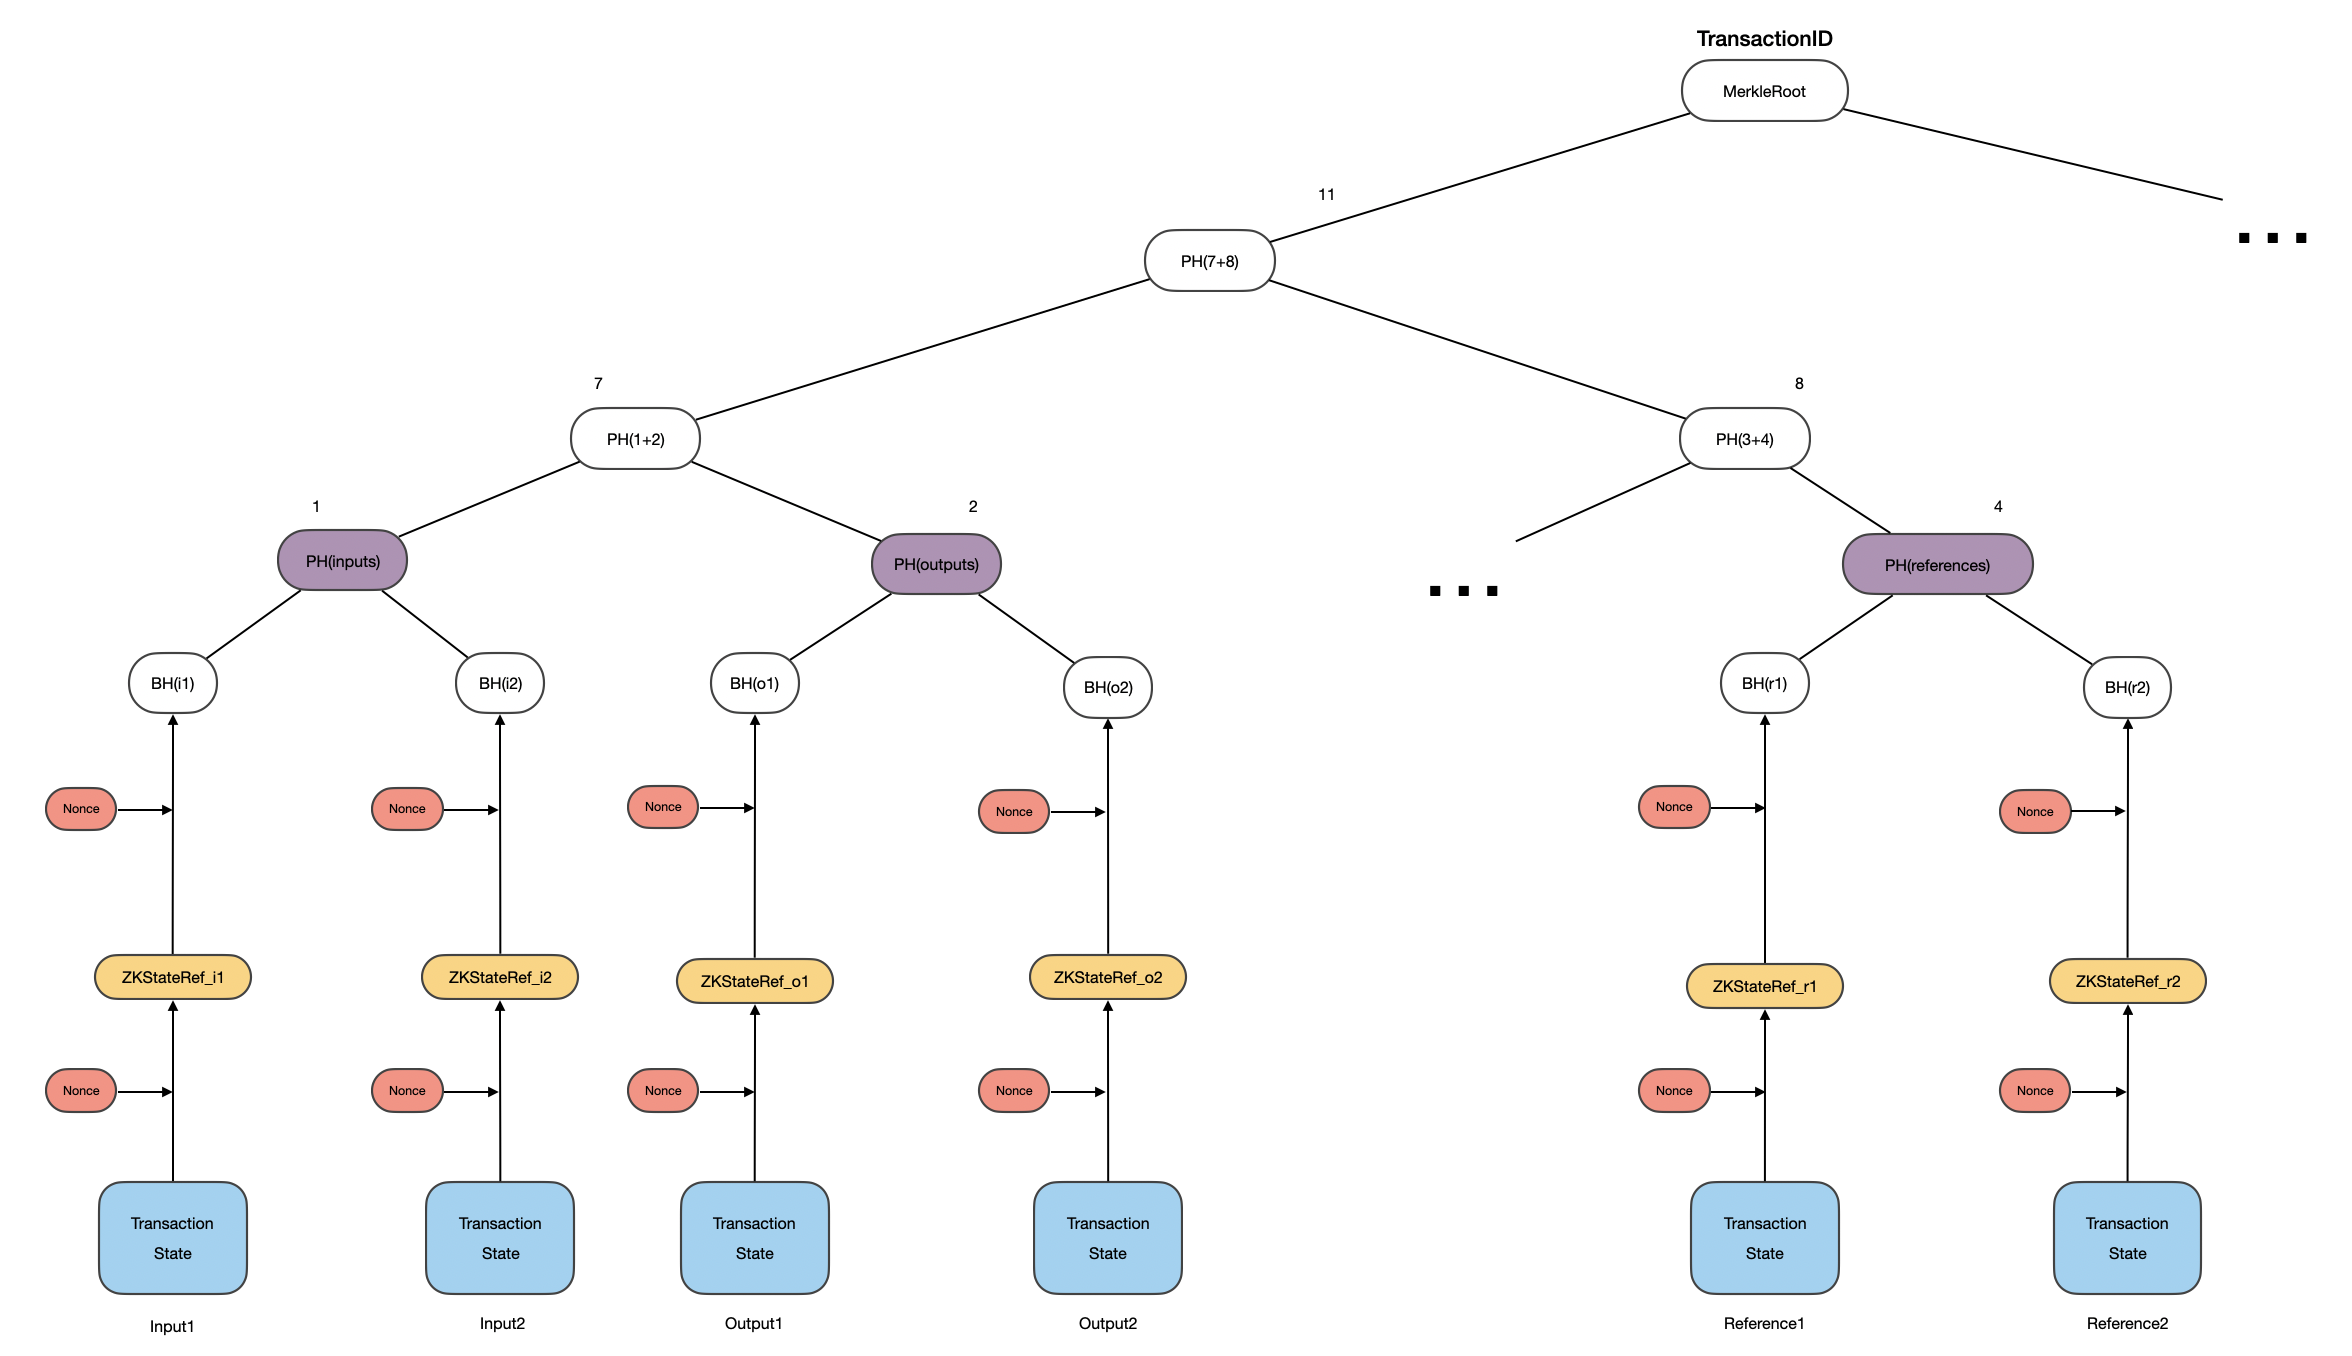
\includegraphics[width=\textwidth]{Appendix1/images/tree_ts}
\caption{Merkle Tree representation of a transaction with \texttt{Transaction State} and \texttt{ZKStateRef}.}
\label{fig:tree_ts}
\end{figure}

A \texttt{Transaction State} consists of following attributes:
\begin{itemize}
\item \texttt{data},
\item \texttt{contract},
\item \texttt{notary},
\item \texttt{encumbrance},
\item \texttt{constraint}
\end{itemize}

We can compute ZKStateRef as
\begin{align}
ZKStateRef &= Hash(nonce \concat state\_fields), \text{ s.t.} \\
state\_fields &= data \concat contract \concat notary \concat encumbrance \concat constraint \nonumber
\end{align}
\noindent and the leaf hash as
\begin{align}
LeafHash &= Hash(nonce \concat ZKStateRef).
\end{align}

Now, considering that the nonce used in the computation of ZKStateRef and LeafHash is the same, the question that we need to answer is that can a malicious party obtain meaningful information about the \texttt{Transaction State} given the public values ZKStateRef, LeafHash, and the computation of the LeafHash?
In this scenario, the malicious party (which is notary in our case) is asked to validate LeafHash by repeating the computation $LeafHash = Hash(nonce || ZKStateRef)$.
This is a reasonable scenario in our design, since the notary is asked to validate a filtered Merkle tree.
The filtered tree that the notary is going to validate is illustrated in Figure~\ref{fig:filtered_tree_ts}.

\begin{figure}[ht]
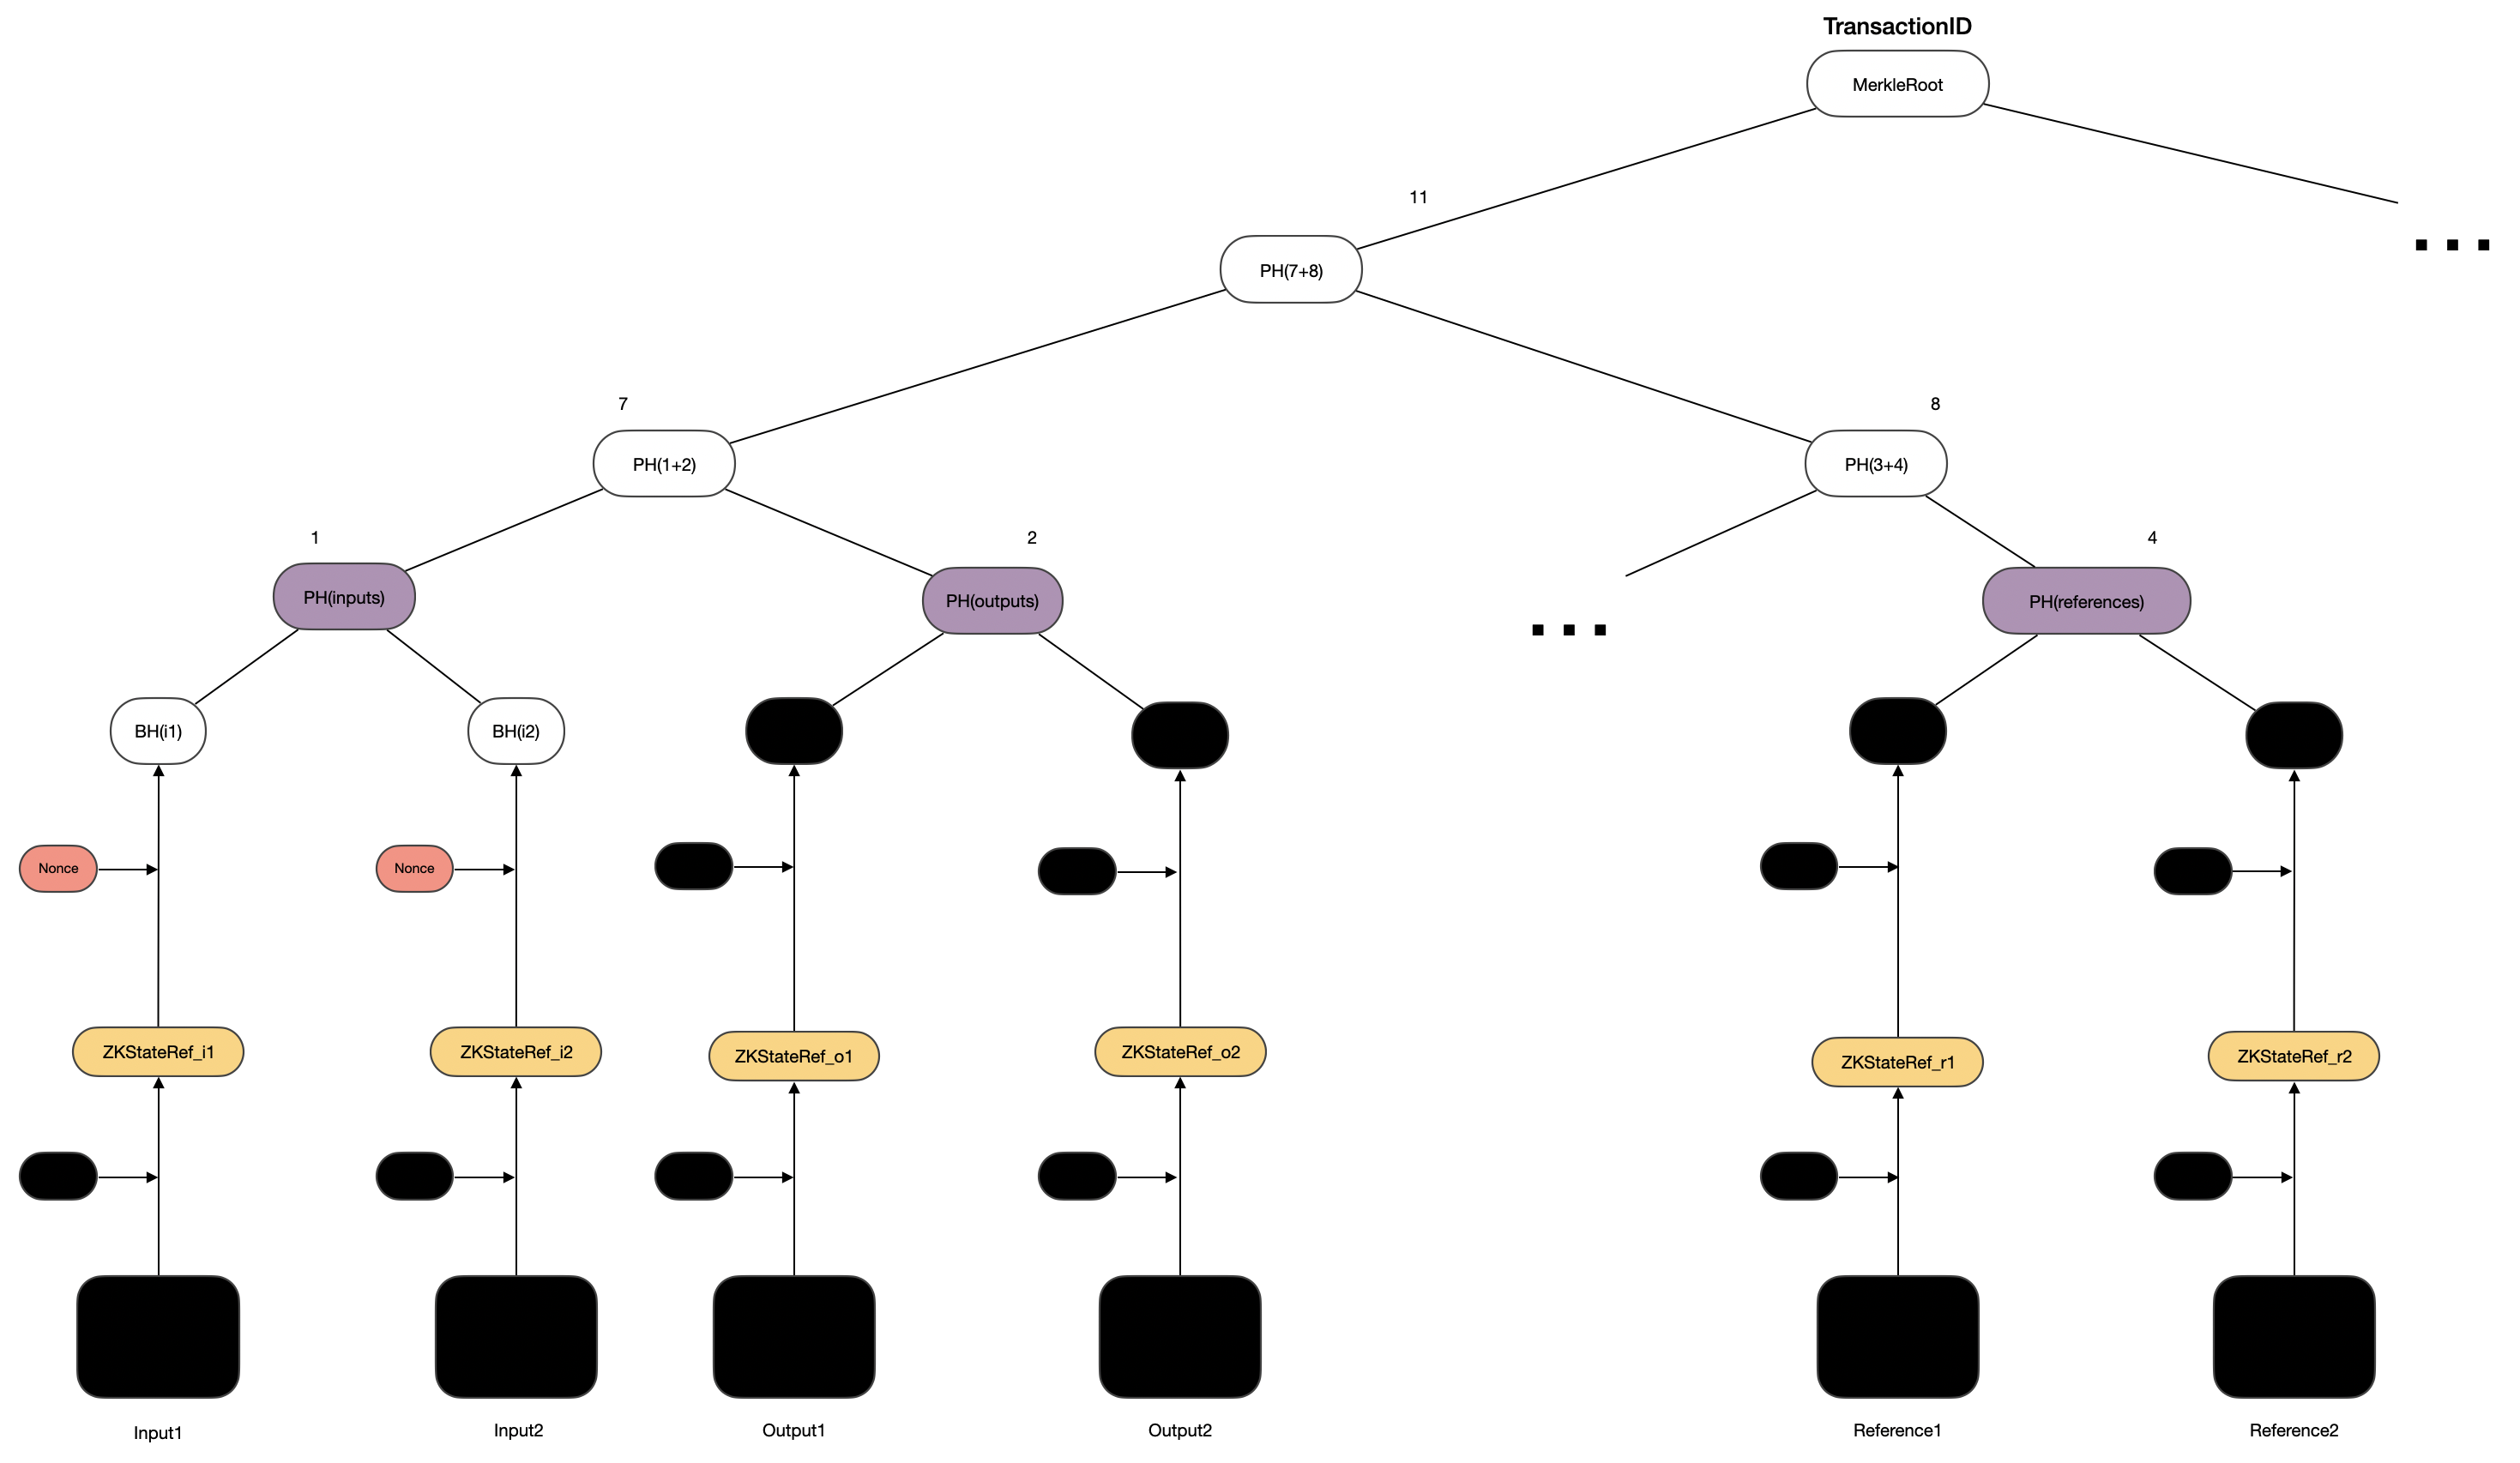
\includegraphics[width=\textwidth]{Appendix1/images/filtered_tree_ts}
\caption{Filtered Merkle Tree representation of a transaction that is validated by the notary.}
\label{fig:filtered_tree_ts}
\end{figure}

In such a scenario, the notary has access to LeafHash, nonce, and ZKStateRef.
Knowing nonce, the difficulty of applying a pre-image attack on $ZKStateRef = Hash(nonce || state\_fields)$ depends on the attacker knowing the contract logic and State object structure (which they will, because they need to know which ZKP circuit to use, so they know the contract).
Knowing the structure, they can make reasonable/educated guesses on the field values of the state based on the contract business logic.

Then, the next question is how can we compute a unique nonce for ZKStateRef without incurring too much additional cost.
We consider three options for that:

\begin{enumerate}
\item Change the order in the computation of nonce such that:
\begin{align}
LeafHash\_nonce &= Hash(privacySalt \concat groupIndex \concat elementIndex) \\
ZKStateRef\_nonce &= Hash(groupIndex \concat elementIndex \concat privacySalt)
\end{align}
\item Use the un-hashed version of nonce in the computation of ZKStateRef (it will be in the proof circuit and won't be revealed any way)
\begin{align}
ZKStateRef\_nonce = privacySalt \concat groupIndex \concat elementIndex
\end{align}
\end{enumerate}

\includesvg[width=\textwidth]{Appendix1/images/fig1}

Some more info. And more.
























\begin{itemize}
\item include glossary 
\end{itemize}

\appendix

\chapter*{Design Choices}

\subsection{Transaction representation:Merkle Tree vs Concatenation}

\subsection{Selection of Nonce for ZKStateRef}

\textbf{Problem:} ZKStateRef can be computed as $\text{ZKStateRef} = Hash(\text{Transaction State})$.
However, this computation is not resistant to pre-image attacks and collisions.

A solution to this problem is adding a nonce in computation such that $\text{ZKStateRef} = Hash(\text{nonce} \concat \text{Transaction State})$, which can prevent such attacks.
However, generating a nonce in Corda requires to perform a hash operation which is a costly operation in ZK circuits.
As an alternative, \textit{can we use the same nonce that is generated for the hashing of component elements?}

Before answering this question, we provide some information about the data that is used in the computation of ZKStateRef.
We compute ZKStateRef for input, output, and reference components.
Each element in these component groups are a \texttt{ZKStateAndRef} object which consists of a \texttt{Transaction State} and \texttt{ZKStateRef}.
Figure~\ref{fig:tree_ts} shows the relation between each object.

\begin{figure}[ht]
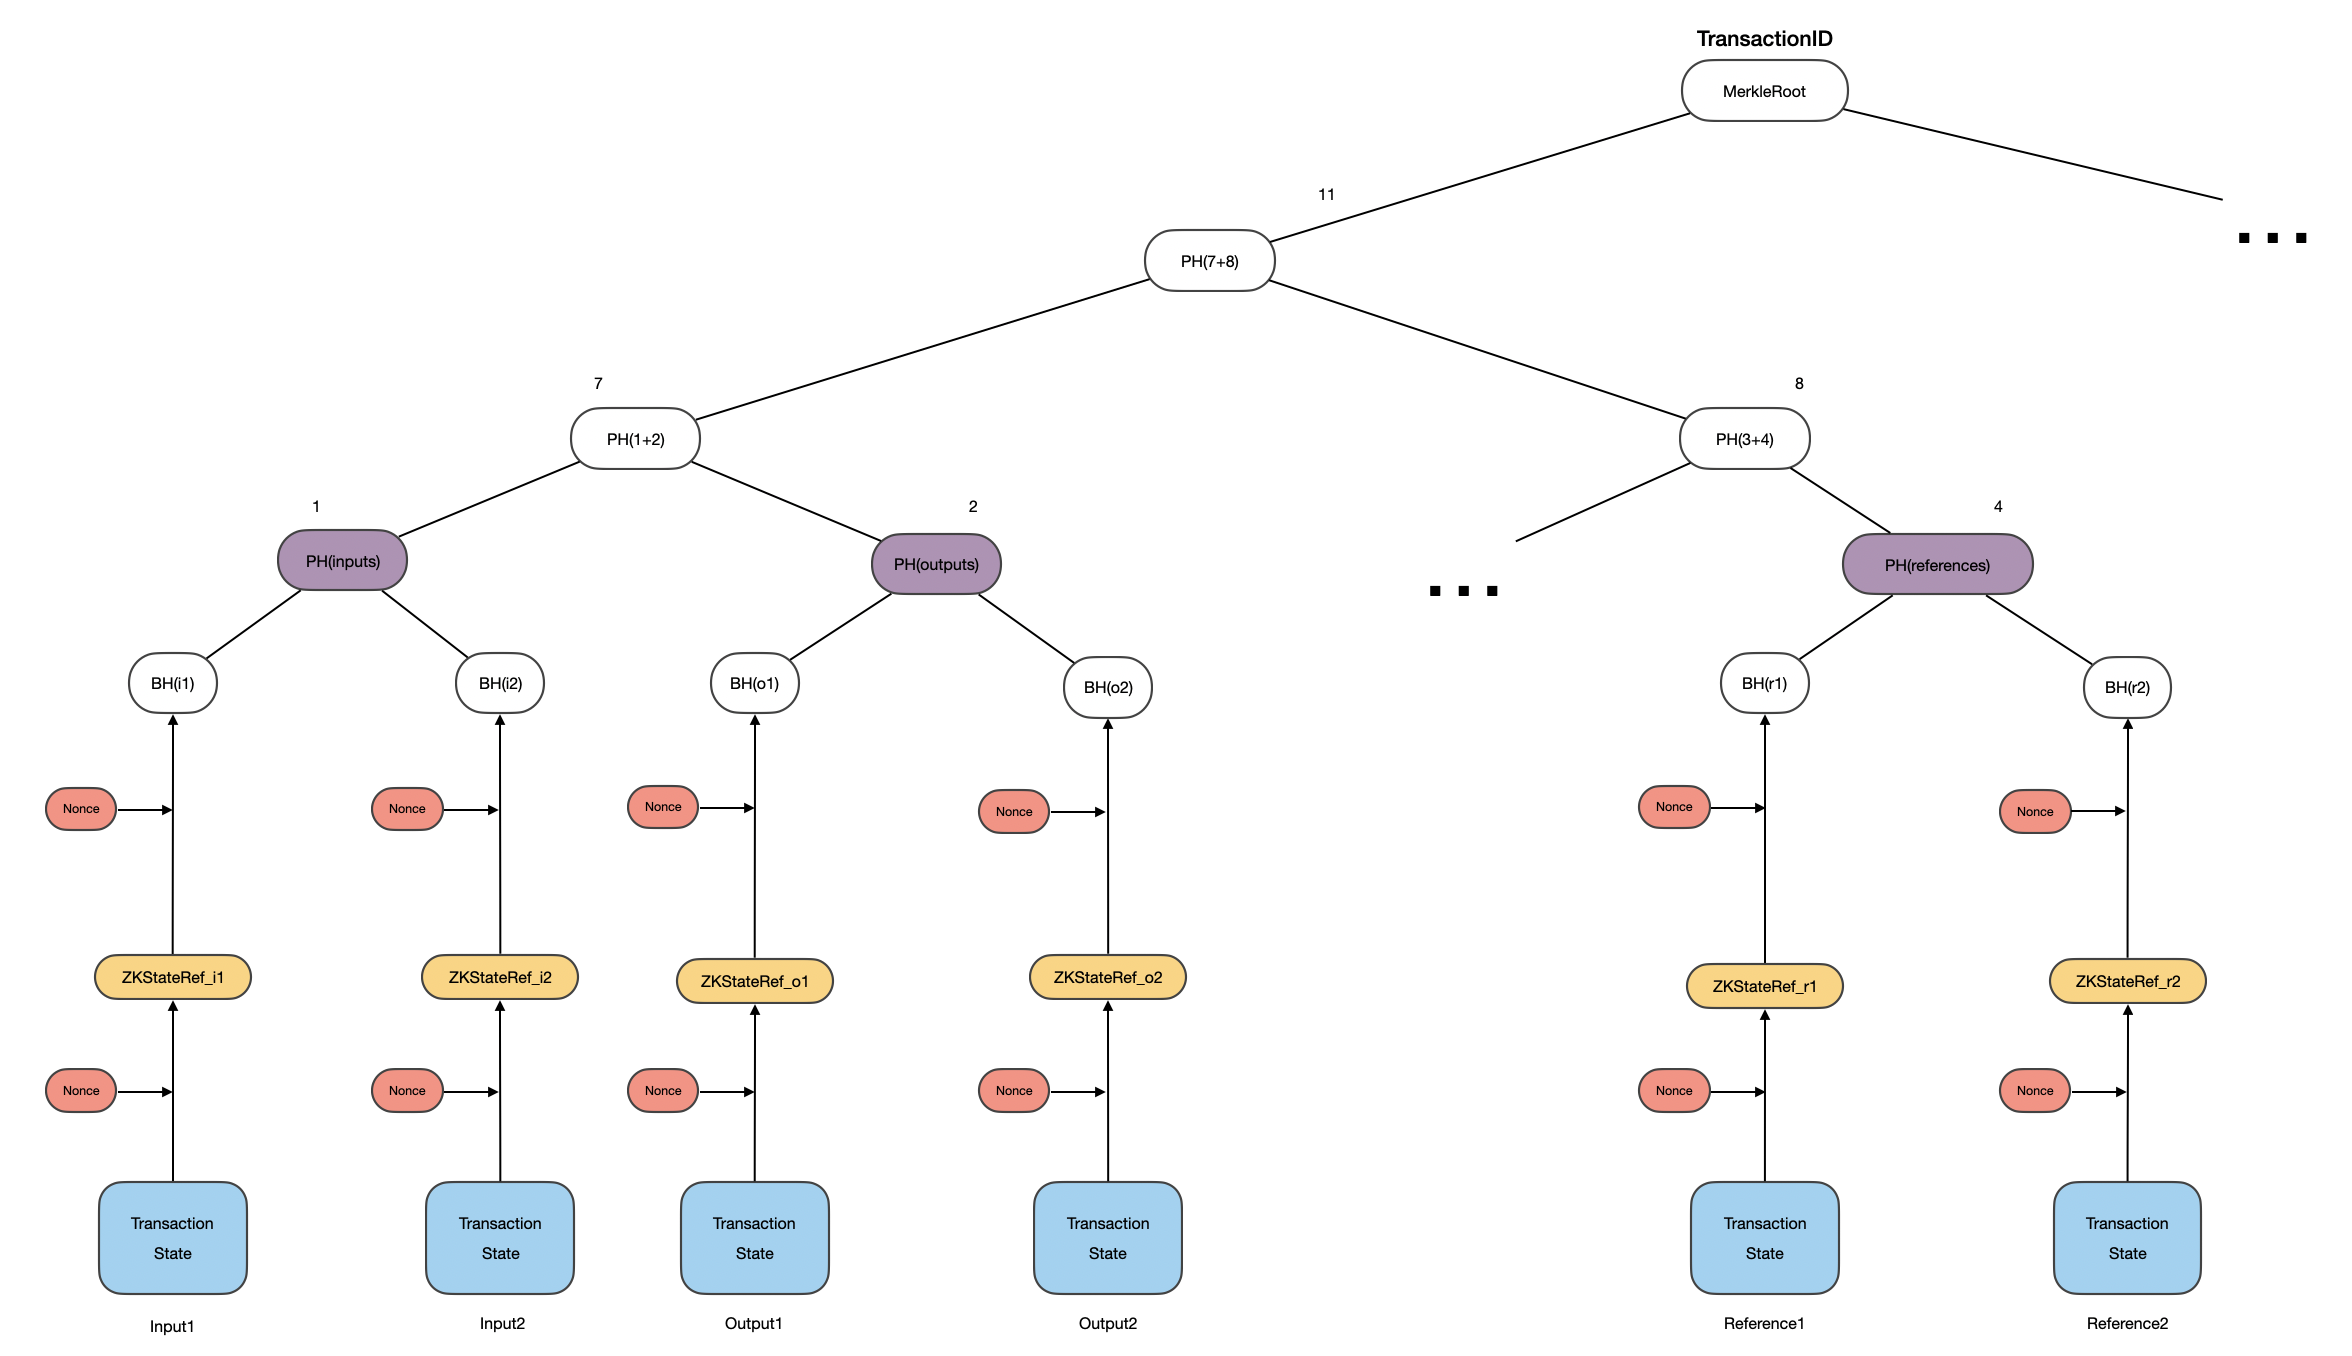
\includegraphics[width=\textwidth]{Appendix1/images/tree_ts}
\caption{Merkle Tree representation of a transaction with \texttt{Transaction State} and \texttt{ZKStateRef}.}
\label{fig:tree_ts}
\end{figure}

A \texttt{Transaction State} consists of following attributes:
\begin{itemize}
\item \texttt{data},
\item \texttt{contract},
\item \texttt{notary},
\item \texttt{encumbrance},
\item \texttt{constraint}
\end{itemize}

We can compute ZKStateRef as
\begin{align}
ZKStateRef &= Hash(nonce \concat state\_fields), \text{ s.t.} \\
state\_fields &= data \concat contract \concat notary \concat encumbrance \concat constraint \nonumber
\end{align}
\noindent and the leaf hash as
\begin{align}
LeafHash &= Hash(nonce \concat ZKStateRef).
\end{align}

Now, considering that the nonce used in the computation of ZKStateRef and LeafHash is the same, the question that we need to answer is that can a malicious party obtain meaningful information about the \texttt{Transaction State} given the public values ZKStateRef, LeafHash, and the computation of the LeafHash?
In this scenario, the malicious party (which is notary in our case) is asked to validate LeafHash by repeating the computation $LeafHash = Hash(nonce || ZKStateRef)$.
This is a reasonable scenario in our design, since the notary is asked to validate a filtered Merkle tree.
The filtered tree that the notary is going to validate is illustrated in Figure~\ref{fig:filtered_tree_ts}.

\begin{figure}[ht]
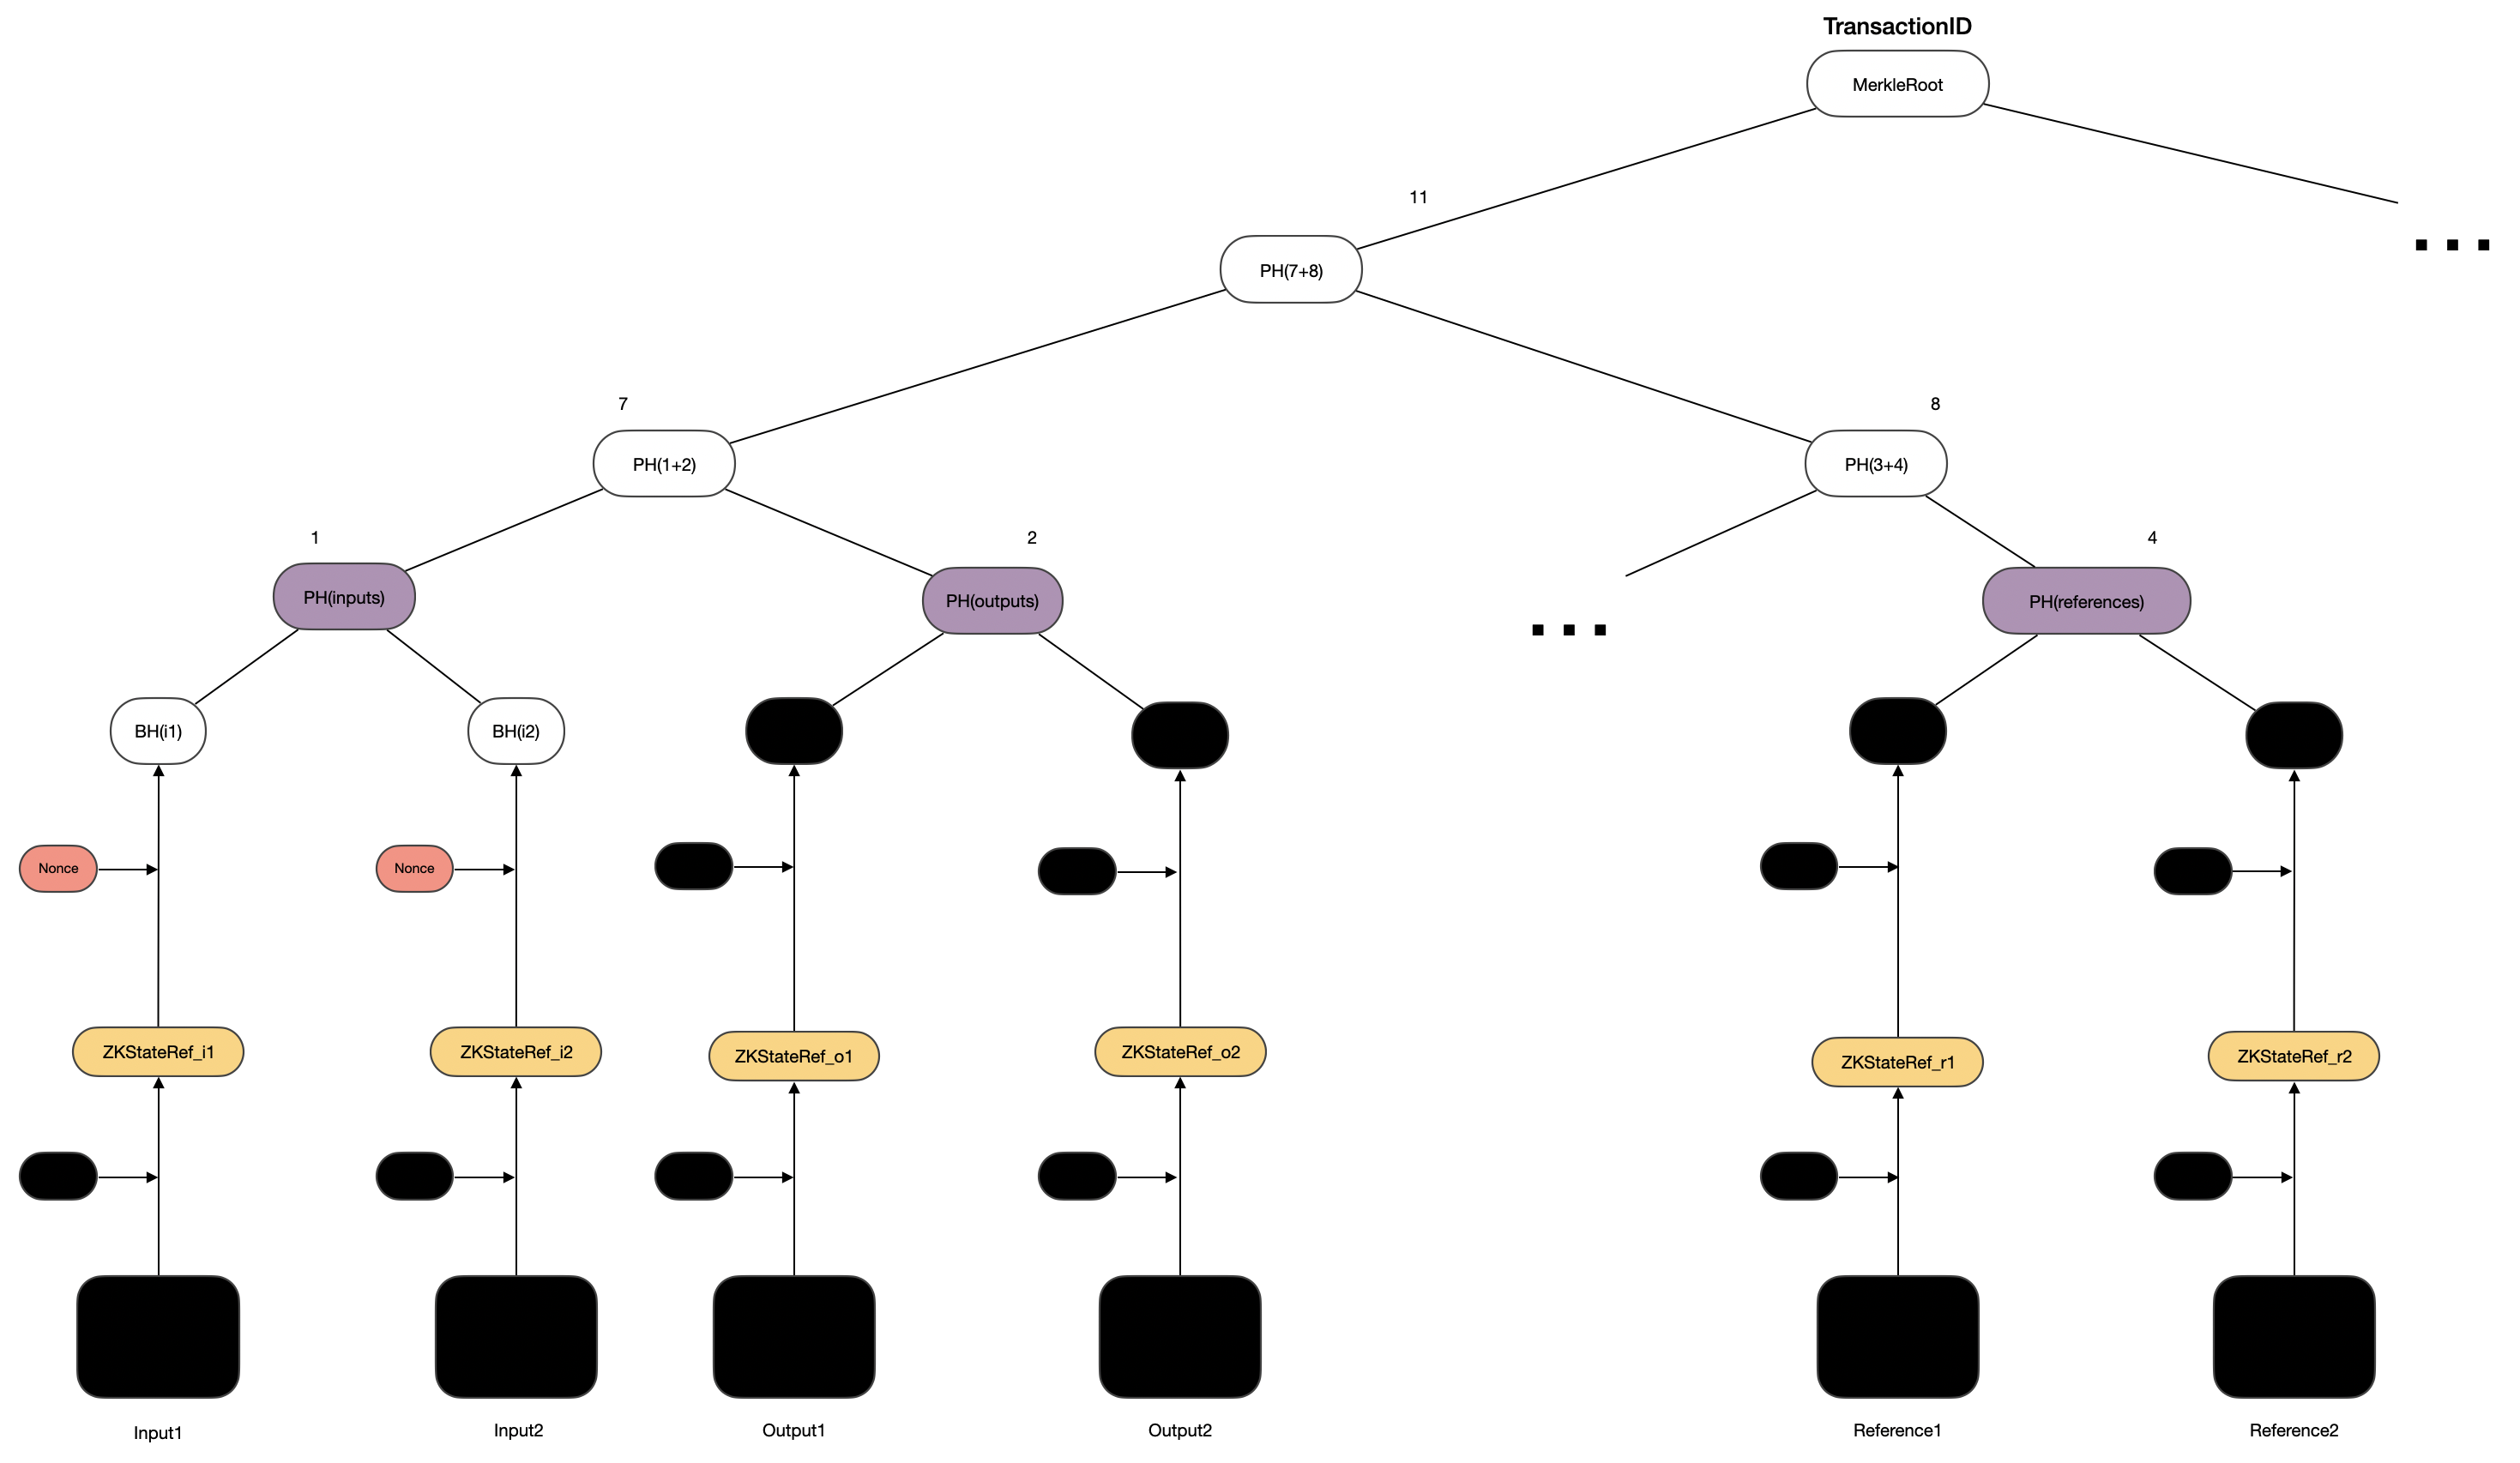
\includegraphics[width=\textwidth]{Appendix1/images/filtered_tree_ts}
\caption{Filtered Merkle Tree representation of a transaction that is validated by the notary.}
\label{fig:filtered_tree_ts}
\end{figure}

In such a scenario, the notary has access to LeafHash, nonce, and ZKStateRef.
Knowing nonce, the difficulty of applying a pre-image attack on $ZKStateRef = Hash(nonce || state\_fields)$ depends on the attacker knowing the contract logic and State object structure (which they will, because they need to know which ZKP circuit to use, so they know the contract).
Knowing the structure, they can make reasonable/educated guesses on the field values of the state based on the contract business logic.

Then, the next question is how can we compute a unique nonce for ZKStateRef without incurring too much additional cost.
We consider three options for that:

\begin{enumerate}
\item Change the order in the computation of nonce such that:
\begin{align}
LeafHash\_nonce &= Hash(privacySalt \concat groupIndex \concat elementIndex) \\
ZKStateRef\_nonce &= Hash(groupIndex \concat elementIndex \concat privacySalt)
\end{align}
\item Use the un-hashed version of nonce in the computation of ZKStateRef (it will be in the proof circuit and won't be revealed any way)
\begin{align}
ZKStateRef\_nonce = privacySalt \concat groupIndex \concat elementIndex
\end{align}
\end{enumerate}

\includesvg[width=\textwidth]{Appendix1/images/fig1}

Some more info. And more.
























\end{document}
